\chapter*{Úvod}

Webové technologie procházejí velkými evolučními proměnami. Internet
už není ono nové a neprobádané místo jako v~90. letech 20.
století, ale naopak se stal běžnou a často i nepostradatelnou
součástí života obyčejných lidí. Technologie se posunují vpřed
jednotně na základě konsensu lídrů trhu, aplikace se přesouvají
z~operačního systému do prohlížeče a vyvíjí se pro ně uživatelská
rozhraní s~ohledem na běžné lidi. Ti se vlastně dostali do středu
veškerého zájmu. Jestliže dříve byl internet místem spíše pro
technicky založené, nyní se snaží oslovit širokou veřejnost.

Různé zajímavé služby otevřeně poskytují svá data a na těch se staví
aplikace s~dříve nepředstavitelnými komplexními funkcemi. Nejlépe to lze vidět
asi na mapách, které prošly neskutečným vývojem a dnes díky nim (když
zmíním jen zlomek jejich možností) například pohodlně naplánujete
cestu autem, zjistíte počasí v~dané lokalitě, vyhledáte nej\-bližší
pekárnu, nebo si prohlédnete fotografie jiných lidí z~míst, kam na
léto plánujete dovolenou. Na základě takových online map vznikají
mnohé specializované služby -- z~těch nej\-zajímavějších v~českém
prostředí bych zmínil například server bezrealitky.cz, jenž na
mapových podkladech zobrazuje realitní objekty. Nechal jsem se
inspirovat a na základě map jsem i já postavil systém, který využívá
mnoha otevřeně nabízených služeb a integruje je do komplexní aplikace
s~užitkem pro běžného uživatele.

Evidencí geografických tras uživatele je tedy myšlena webová aplikace,
jež umožňuje uživateli interaktivně zaznačit do mapových podkladů trasu,
kterou plánuje absolvovat či kterou již absolvoval například na kole,
pěšky, na bruslích nebo během. Nic samozřejmě uživateli nebrání
evidovat i jiné, delší trasy, systém by měl být však primárně určen
pro výše naznačené lokální sportovní využití.

Bakalářská práce se postupně zabývá analýzou současného stavu
možností využití nej\-různějších aplikačních rozhraní a analýzou
možností interoperability programu s~okolím. Na základě těchto
poznatků se snaží ucelit na rozbor pohled, specifikovat zadání a
nabídnout rámcový návrh řešení. Ten v~dalších kapitolách zpracovává
podrobněji a postupně přejde do obeznamování čtenáře s~detaily
implementace projektu. V~poslední krátké kapitole popisuje podmínky,
v~nichž byl program vyvíjen a testován. Závěr práce pojednává
o~jejích přínosech a zmiňuje vizi, jak implementovanou aplikaci
rozvíjet do budoucna.

Celkově chce práce uvést čtenáře do problematiky stavby webové
aplikace na základě různých API, osvětlit mu pojmy související
s~problematikou a navést či pomoci při řešení některých tradičních
problémů, pokud by měl zájem podobnou aplikaci vyvíjet.

\chapter{Pojmy Web~2.0 a mashup}\label{mashup}

Dvacáté století nám připravilo univerzální platformu s~obrovským
potenciálem. Lidé spojili inovativní myšlenky z~mnoha směrů informatiky,
vybudovali fungující síť, úspěšně ji rozšířili po celé planetě
a dokázali z~ní vytvořit každodenního pomocníka, bez kterého si život
už příliš představit nedokážeme. Kolem roku 2000 bylo na světě kolem
250~000~uživatelů internetu a toto číslo dále stoupalo exponenciálně
\footnote{Viz \url{http://www.internetworldstats.com/}.}.

Do nového století jsme však stále vstupovali spíše s~pocitem, že
internet je něco nového a že tušíme minimum o~tom, jaké jsou jeho
možnosti. Webové technologie byly celkem nesmělé, statické a pasivní.
Trh s~prohlížeči, hlavními katalyzátory vývoje, byl nestabilizovaný.
Namísto toho, aby velcí hráči internetového trhu spolupracovali a
v~navrhovaných novinkách se pokoušeli o~konsensus, byly technologie
proprietárně uzamykány.

Až dnes se postupně dostáváme do doby, kdy můžeme pracovat
s~relativně jednotně podporovanými technologiemi, kdy se prosazují
spíše otevřená řešení a kdy začínají internetové subjekty
spolupracovat mezi sebou a více využívat možností propojení pomocí
internetu. Evoluce přinesla novou éru webu, brzy pojmenovanou jako
{\it Web~2.0} \cite{web20}. Začaly se objevovat složité interaktivní
aplikace přímo ve webovém prohlížeči, stránky přestaly být izolovanými ostrůvky
statických informací, ale naopak mezi sebou začaly kooperovat,
poskytovat si navzájem data a funkcionalitu. Masivní rozšíření
internetu mezi běžné uživatele podnítilo vznik tzv. {\it sociálních
služeb}, kde mohou lidé sdílet informace mezi sebou a snadno
komunikovat, a také přineslo požadavek na propracovanější a
příjemnější uživatelské rozhraní webových aplikací.

Velmi mnoho nových Web~2.0 služeb dnes nabízí své aplikační
rozhraní (API, {\it Application Programming Interface}) k~volnému
využití. Kombinací těchto API vznikají velmi silné aplikace, postavené
pomocí minima programování a maximálního využití hotové funkčnosti.
Taková architektura se dnes označuje běžně jako mashup (míchanice).

Do kontextu tohoto nového proudu jsem se rozhodl zasadit svou práci a
vytvořit právě výše zmíněný mashup. Má aplikace využívá mnoha služeb a
datových zdrojů poskytovaných otevřeně a online, spojuje je dohromady
a staví na nich novou službu pro běžného netechnického uživatele.
Navíc nabízí dle trendů interaktivní uživatelské rozhraní a snaží se
uživateli poskytnout prostor pro sdílení svých dat s~ostatními.

Zajímavě problematiku mashupů zpracoval ve svém článku
\cite{certodejMashup} český internetový novinář a podnikatel Patrick
Zandl. Na téma API se v~seriálu \cite{misantropApi} rozepsal Martin
Malý.

\chapter{Analýza dostupných veřejných aplikačních rozhraní}

Evidence geografických tras uživatele je aplikací postavenou na
architektuře mashup (viz \ref{mashup}), a proto je výběr API již
z~principu zcela zásadní. S~ohledem na tuto skutečnost problematice
věnuji velký následující úsek práce.

\section{Mapové podklady}\label{vybermap}
V~oblasti mapových technologií na internetu proběhl
v~posledních letech opravdový zlom. Vše začalo 8. 2.
2005 \cite{gmaps}, kdy Google spustil své revolučně zpracované,
interaktivní Google Maps. V~řetězové reakci si postupně i další
provozovatelé online map začali uvědomovat skrytý potenciál této
služby (prodej regionální reklamy, cílená reklama, partnerství
s~jízdními řády apod.) a začali také investovat velké částky do její
modernizace. Na českém internetu navíc vznikly časem tři velké a
velmi kvalitní mapové servery, což je ve světě celkem jedinečný úkaz
a působí ještě unikátněji, přihlédneme-li k~velikosti a významu naší
země.

Ještě v~roce jejich vydání představil Google jako první u~svých
map aplikační rozhraní pro použití mapových podkladů i na jiných
webech. Vydání API se setkalo s~obrovským ohlasem \cite{gmapsSuccess}
a nadobro změnilo web, jak jsme ho znali. Po celém internetu se začaly objevovat
interaktivní mapy -- od jednoduchých orientačních výřezů po aplikace
na mapách kompletně založené. Konkurence ani nyní nespala a odpověděla
svými vlastními API.

V~následujících odstavcích se pokusím popsat specifika, výhody a
nevýhody jednotlivých mapových podkladů, jež jsem bral pro svou práci
v~úvahu. Je nutné podotknout, že samotných mapových serverů je mnohem
více (např. Mapy iDNES.cz, Yahoo! Maps, Ask.com Maps \& Directions,
Multimap, NAVTEQ Map24, Bing Maps, aj.), ale nelze jejich služeb využít,
protože poskytované datové podklady nejsou dostatečné pro Českou
republiku, API vůbec nenabízejí, nebo má velmi omezené možnosti. Také
jsem vynechal možnost získat geografická data jejich zakoupením přímo od dodavatelů.

\subsection{Google Maps společnosti Google}
Průkopník v~oblasti online map, Google, nabízí samozřejmě mapový
server i API již hodně dlouho, takže jeho služby jsou v~mnoha směrech
nej\-vyzrálejší. API je pod neustálým vývojem a v~době psaní práce
Google pracuje na jeho třetí
verzi\footnote{V době psaní práce dostupné na
\url{http://code.google.com/intl/cs/apis/maps/documentation/v3/}.}.

Nelze se však nechat unést jeho možnostmi a je nutné zaměřit se i na
jiné rysy, důležité pro tuto práci. Mezi takové patří
například skutečnost, že do češtiny začala být služba lokalizována až
nedávno \cite{googleCesky}.
Dnes je již sice míra integrace map do českého prostředí na velmi
dobré úrovni, ale z~hlediska mapových podkladů má jednu velkou mezeru
-- turistická data. Google poskytuje mapy globálně a proto se mu
v~nich velmi špatně odráží specifika jednotlivých zemí. K~dispozici
jsou sice terénní mapy s~vrstevnicemi, ale neexistuje možnost
zobrazit na nich české turistické trasy a cyklostezky.

\begin{figure}[h]
	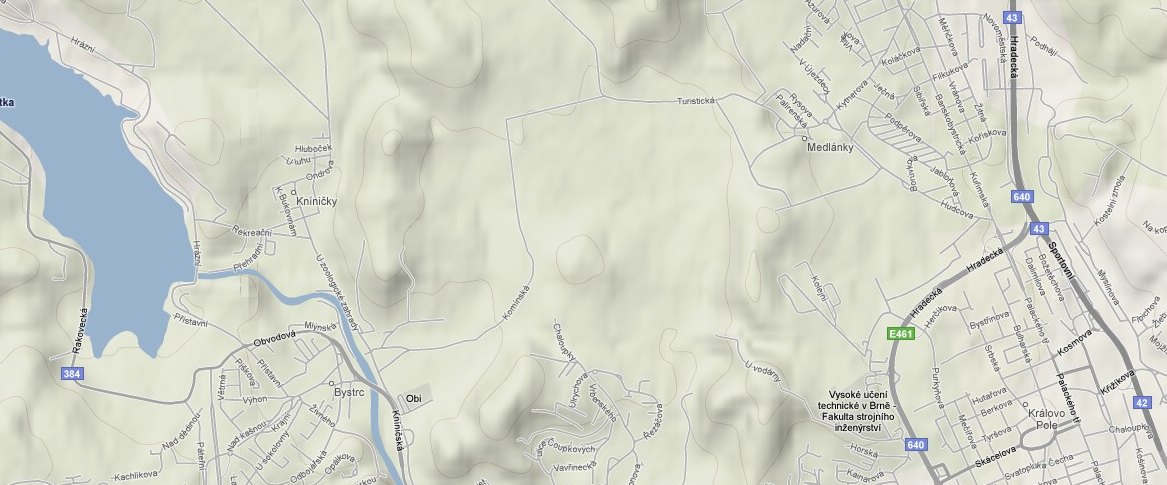
\includegraphics[width=\textwidth, keepaspectratio]{fig/mapagoogle}
	\caption{Náhled na turistickou mapu Google Maps.}
	\label{obrGoogleMap}
\end{figure}

Jinak jsou podklady kvalitní, i když někdy méně přesné, než
u~lokálních mapových služeb. Google používá kombinaci několika zdrojů
geografických map, přičemž většinu českých podkladů získává od
dodavatele GEODIS Brno. Předností map je samozřejmě dostupnost
podkladů pro celý svět a lákavá je rovněž představa možného budoucího 
napojení aplikace např. v~podobě vrstvy na program Google
Earth\footnote{Google Earth je multiplatformní program společnosti
Google představující virtuální online glóbus. Nabízí pohled na zemi
jako z~družice, virtuální 3D modely některých měst, detailní snímky
zajímavých míst po celém světě a umožňuje překryv mapových podkladů
tzv. vrstvami poskytujícími další informace. Google jej nabízí
v~několika variantách, z~nichž základní je zdarma.}.

\subsection{Mapy.cz společnosti Seznam.cz}
Mapy.cz byly prvním ryze českým projektem v~oblasti nových online map
a dodnes jsou lídrem lokálního trhu. Stejně jako za Google Maps stojí
i za těmito mapami silná společnost. Budoucnost serveru a případný
další vývoj API je celkem jistý. Seznam.cz se na rozdíl od všech
ostatních českých portálů profiloval po vzoru Google spíše do
společnosti, jež svou budoucnost spojuje s~technologickým pokrokem,
než do mediálního vydavatelství jako například Centrum Holdings.
Odhadnutelné záměry potvrdili uveřejněním zprávy o~vývoji nového
API \cite{apiSeznam} v~době tvorby této práce.

Současný stav API je ale celkem nešťastný. Aplikační rozhraní nabízí
jen omezenou škálu funkcí, omezené mapové podklady oproti službě
Mapy.cz a samotná práce s~funkcemi API působí na vývojáře poněkud
těžkopádně. Jeho licenční podmínky navíc nejsou tak volné jako
u~ostatních API a požadují registraci klíče nikoliv na doménu, ale
přímo na unikátní URI, kde se má mapa nacházet. To jej pro tvorbu
složitější aplikace prakticky vyřazuje ze hry. V~podmínkách je také
omezení na 1000 zobrazení denně a zákaz provozu map pro komerční
užití, což v~ranné fázi projektu není velkou překážkou, ale pro
budoucí rozvoj projektu ano.

Nové API čtvrté verze vyvíjí v~Seznam.cz Ondřej Žára, autor známého
nástroje pro tvorbu databázových schémat, {\it WWW SQL
Designer}\footnote{Dostupné na
\url{http://code.google.com/p/wwwsqldesigner/}.}, což je určitou zárukou kvality. Bohužel rozhraní je zatím stále dost
nestabilní a podle jeho slov na diskusi k~projektu ani jemu stále
ještě nejsou známy nové licenční podmínky.

\begin{figure}[h]
	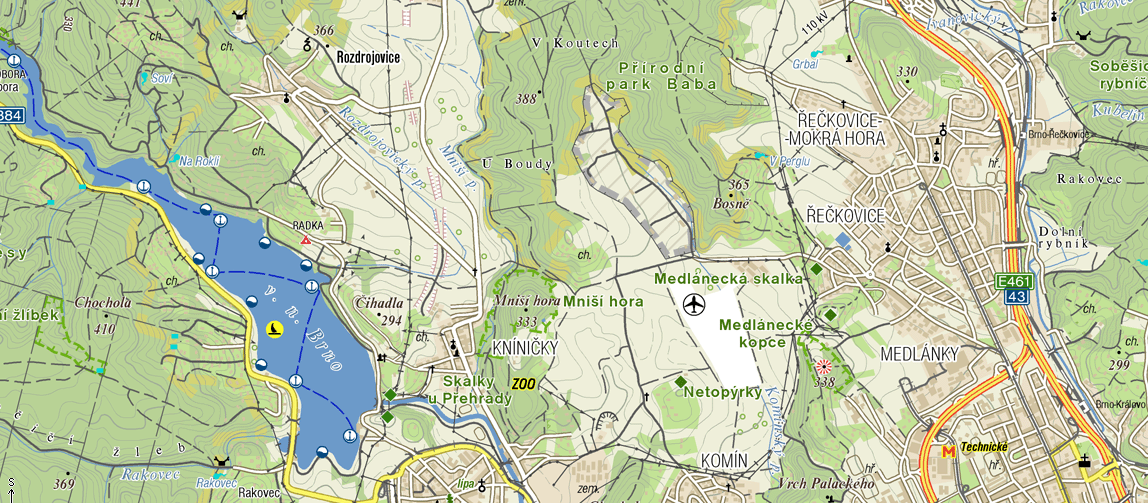
\includegraphics[width=\textwidth, keepaspectratio]{fig/mapaseznam}
	\caption{Náhled na turistickou mapu Mapy.cz.}
	\label{obrSeznamMap}
\end{figure}

Mapy.cz jsou připraveny kombinací geografických dat od PLANstudio a
GEODIS Brno. Turistická mapa je nej\-kvalitnější podobnou mapou na českém
internetu\footnote{Za její asi nej\-podstatnější nevýhodu by se dala
chápat absence velkého měřítka. Turistickou mapu lze na rozdíl od té
na Amapy.cz přiblížit jen do poměrně omezené podrobnosti.}. Seznam.cz
ji poskytuje na základě dat společnosti SHOCart, známou svými
papírovými turistickými a cyklistickými publikacemi. Je škoda, že
nepoužitelné API v~tomto případě brání využít tak kvalitní podklady.

\subsection{Amapy.cz společnosti Centrum Holdings}
Amapy.cz se na svět dostaly v~roce 2006 pod hlavičkou portálu
Atlas.cz. Ihned od představení (viz \cite{amapy}) bylo jasné, že se
s~nimi musí na českém trhu počítat -- zpracování bylo profesionální a spolu s~mapami přišlo
i první, na funkce bohaté, dobře dokumentované české mapové API. Vývoj
však postupně ustával a po tom, co byl Atlas.cz sjednocen
s~Centrum.cz pod hlavičku Centrum Holdings, nelze již kolem API
pozorovat vůbec žádnou činnost ze strany provozovatele. Celou službu
původně zpracoval Daniel Steigerwald, který tyto informace pro mou
práci potvrdil
\footnote{Viz \url{http://twitter.com/steida/statuses/2211073537}.}.

\begin{figure}[h]
	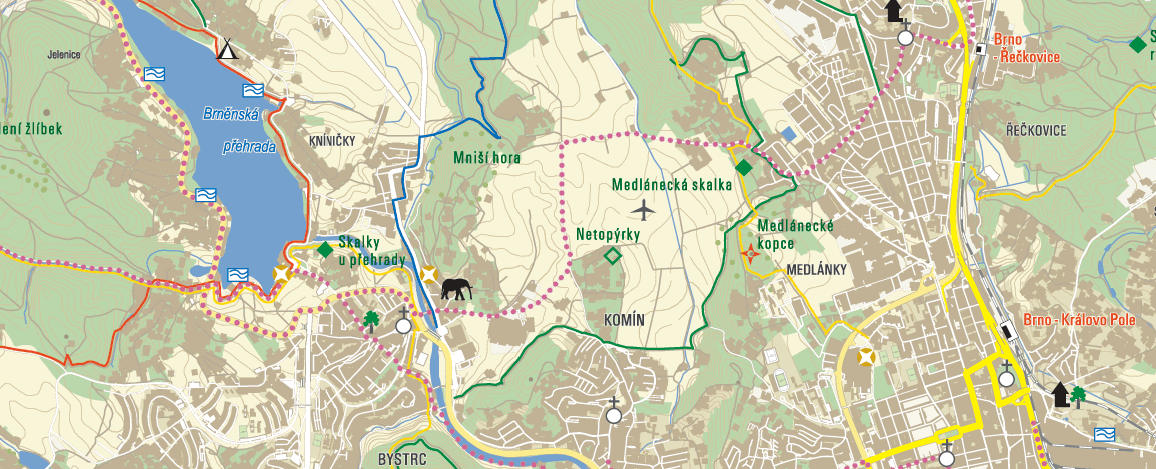
\includegraphics[width=\textwidth, keepaspectratio]{fig/mapacentrum}
	\caption{Náhled na turistickou mapu Amapy.cz.}
	\label{obrCentrumMap}
\end{figure}

API je však opravdu velmi dobře použitelné a mapové podklady
kvalitní, připravené ve spolupráci s~firmou DPA. I~přes API lze
dokonce zobrazovat vrstvy s~turistickými a cyklistickými značkami a už i
zcela základní mapa disponuje vrstevnicemi. Aplikační rozhraní nabízí
funkce, jež nelze najít ani u~Google Maps API a podporuje několik
souřadnicových systémů naráz, což je výhodné při spolupráci s~jinými
službami (každá požaduje body v~jiném formátu).

Specifikem API je integrovaný JavaScriptový framework MooTools 1.11.
Výhodou je, že po vložení API do stránky lze přímo využít všech výhod
frameworku a není nutné nějaký připojovat dodatečně. Nevýhodou je
nemožnost vlastního výběru frameworku a také ustrnutí vývoje API,
protože v~důsledku toho nebyl průběžně framework obnovován a zůstal
v~API ve verzi 1.11, ačkoliv během psaní práce byl vydán již ve
velmi odlišné verzi 1.2.3.

\subsection{Otevřený projekt OpenStreetMap}
OpenStreetMap je otevřený projekt, který se snaží vytvořit volně
dostupná geografická data. Získává je integrací dat z~různých zdrojů
a především individuálním sběrem dat pomocí GPS zařízení. Mnoho
institucí, organizací a dokonce i firem uvolnilo svá data pod licencí
kompatibilní s~OpenStreetMap, aby tomuto projektu pomohli.

Kvalita mapových podkladů pro ČR však není zrovna nej\-lepší a
pro účely aplikace se nehodí ani forma jejich zobrazení. Mapy sice
obsahují například polohu sloupů elektrického vedení nebo přesné
hranice lesů, vrstevnice nebo turistické značky a cyklostezky však
nepodporují.

OpenStreetMap je zajímavý počin a do budoucna možná perspektivní, ale
o~jeho použití ve své práci jsem příliš neuvažoval. Uvedl jsem jej
pro úplnost jako alternativní a otevřený zdroj geografických dat,
jenž by v~budoucnosti mohl nabýt na relevanci.

\section{Výškový profil}\label{vyskovyProfil}
\subsection{Nadmořská výška}\label{vyskopis}
Existují de facto dva hlavní zdroje dat o~nadmořské výšce.
Český Výškopis.cz (celosvětově pod názvem Topocoding.com) a potom
jeden ze škály zdrojů dostupných na GeoNames.org.

Výškopis.cz na svých stránkách představuje ukázky JavaScriptového API
přímo na všech třech českých mapových systémech a má dokonce přímou funkci pro
vygenerování výškového profilu Na druhou stranu má však mírně
omezující podmínky (počet požadavků za 24 hodin může být
limitován na 10000) a hlavně nejsou nikde k~dispozici nejen kontaktní
údaje, ale ani název provozovatele. Nicméně služba funguje a
její topografická data jsou kvalitní kombinací SRTM3 a GTOPO30 -- pro
většinu území mají horizontální rozlišení kolem 90 metrů
\footnote{Viz popis služby dostupný na
\url{http://www.vyskopis.cz/index.php?option=com_content&task=view&id=1&Itemid=9}.}.

GeoNames.org poskytují pouze data
z~GTOPO30, takže dosahují rozlišení asi jednoho kilometru
\footnote{Viz dokumentace k~API dostupná na
\url{http://www.geonames.org/export/web-services.html\#gtopo30}.}. GeoNames.org
jsou široce využívaným a známým \footnote{Seznam uživatelů obsahuje společnosti
jako BBC, Adidas nebo Nike -- viz \url{http://www.geonames.org/users.html}.}
poskytovatelem nej\-růz\-něj\-ších dat, takže jej zřejmě lze považovat za
spolehlivý.

\subsection{Grafy}\label{grafy}
Pro zobrazení výškového profilu uživateli je potřeba mít možnost
dynamicky vygenerovat spojnicový graf. Dalo by se použít přímé funkce
aplikačního rozhraní služby Výškopis.cz (viz \ref{vyskopis}), ale
výsledná podoba jejich grafu není příliš parametrizovatelná a navíc by
jeho implementace vázala důležitou část aplikace na jedno konkrétní API.

Profil se dá pomocí výškopisných dat generovat jednoduše i
s~vlastními nástroji, pokud má aplikace k~dispozici potřebná data na
trase. Vybíral jsem mezi povedenou PHP knihovnou pro generování
grafů {\it pChart}, interaktivní Flash knihovnou {\it Open Flash Chart
2} a vzdáleným REST rozhraním {\it Google Chart API} (viz \ref{rest}).

\section{Geocoding}\label{geocoding}
Výrazem {\it geocoding} se rozumí proces vyhledání zeměpisných
souřadnic na základě jiných geografických dat jako například adresa
nebo PSČ.

Veřejně tuto službu nabízí v~požadované kvalitě dva subjekty --
Google v~rámci svého Google Maps API a Yahoo. První zmiňované má
velmi dobrou síť údajů pro Českou republiku, druhé naopak spíše
omezenou.

\section{Obraz z~terénu}
\subsection{Fotografie}
V~oblasti API k~fotografiím, u~nichž lze vyčíst data o~poloze místa
jejich vzniku, existuje snad pouze jediný zdroj, Panoramio. To je
služba, kam se mohou uživatelé zaregistrovat, nahrávat své fotografie
a následně jim přiřazovat polohu na mapě. Stala se po svém vzniku
rychle velmi populární \cite{panoramio} a se svým API je zřejmě bezkonkurenční,
jelikož jsem na žádnou jinou alternativu nenarazil. Panoramio bylo
v~roce 2008 koupeno společností Google.

\subsection{Webkamery}
Existují mnohé služby zabývající se zobrazováním
veřejných webkamer jak u~nás, tak i ve světě. Bohužel velmi málo
z~nich nabízí přímé API. Nejblíže k~tomu z~českých je Webcams.cz,
které nabízí export dat na základě domluvy. Velmi dobrou
síť kamer pro ČR a navíc výborné API jsem však našel
u~Webcams.travel, globální služby využívané například i na Google
Maps.

\section{Počasí}
Při hledání API k~informacím o~počasí lze narazit na mnohá výborná
rozhraní i data, avšak většinou pouze pro USA. Z~celosvětových služeb
lze jmenovat především Weather.com s~přístupem pro vývojáře. Pracuje
však na základě svých jednoznačných identifikátorů k~meteostanicím a
ty není příliš dobře možné programově získat ze zeměpisných
souřadnic. Yahoo Weather poskytuje jednoduché API, ale data má
z~Weather.com, takže počasí vrací oproti těm samým problémovým kódům.

Světové zdroje nebývají zdaleka tak přesné v~datech jako české.
Z~našich poskytovatelů lze najít dva hlavní zdroje dat o~počasí,
Meteopress a ČHMÚ\footnote{Český hydrometeorologický ústav.}. Oba
však svá data nikde nenabízejí v~podobě API a pokud ano, jedná se
spíše o~placenou službu. Jediný server s~aplikačním rozhraním je
In-počasí.eu s~daty od ČHMÚ. Na požádání odhalí adresy XML souboru,
jenže v~něm se nachází pouze jednoduchá globální předpověď pro ČR bez
místního rozdělení.

Marné hledání jsem skončil u~dvou dalších poskytovatelů dat
o~počasí -- Google a GeoNames.org. Na webu lze dohledat zmínky o~Google
Weather API, ale bližší přezkoumání nás přivádí ke skutečnosti, že je
to pouze neoficiální kanál bez podpory a dokumentace. Několik lidí si
všimlo, že Google aplikace se svými programovými dotazy na počasí
míří na jednu určitou adresu a že ji lze využít i veřejně, ale ze
strany společnosti neexistuje žádné vyjádření. Poslední šancí tedy
byly GeoNames.org (viz \ref{vyskopis}), které mají dokonce rozhraní se
vstupem v~podobě zeměpisných souřadnic, nicméně ani ty nelze použít, jelikož mají data
pouze z~větších letišť v~ČR a těch je tak málo, že by vrstva
s~těmito údaji v~mé aplikaci neměla příliš velký smysl. 

\section{Užitečná turistická data}\label{poi}
Na mapě lze zobrazovat vrstvy s~tzv. body zájmu, označovanými často
zkratkou POI z~anglického {\it point of interest}.

\subsection{Wikipedia}
Zajímavým zdrojem POI je otevřená encyklopedie Wikipedia, v~níž je
mnoho článků označených zeměpisnými souřadnicemi. Lze tak například
na mapě Jižní Moravy zobrazit k~poloze zámku Lednice detaily z~článku
o~tomto zámku na české (ale i jiné) Wikipedii. Encyklopedie samotná
sice takovou službu přímo nenabízí, ale lze ji najít u~GeoNames.org
jako zcela standardní API.

\subsection{Jiné zdroje POI}
GeoNames.org (viz \ref{vyskopis}) také nabízí API\footnote{Nejen API,
protože všechna data poskytovaná na GeoNames.org si lze dokonce legálně stáhnout a použít
jako vlastní databázi.} ke zřejmě nej\-ucelenější veřejné databázi
ostatních topografických dat. Je to celosvětová a i pro ČR velmi
hustá síť názvů a dalších informací o~významných místech
s~geografickými souřadnicemi a kategorizací podle typu obsahu.

Jediné další API, které mne v~tomto směru zaujalo, bylo to u~služby
Tixik.com, mezinárodního turistického průvodce. Rozhraní vypadá velmi
dobře, ale data jím dodávaná jsou bohužel prakticky nepoužitelná. Na
dotaz se souřadnicemi server neodpoví
informacemi či fotografiemi o~nej\-zajímavějších místech jak
prezentuje, ale řadou příspěvků z~jeho fóra týkajících se okolí
v~blízkosti bodu.

\chapter{Možnosti interoperability aplikace}
Pojem interoperabilita lze vysvětlit jako schopnost vzájemně si
rozumět, vzájemně spolupracovat, dosáhnout vzájemné součinnosti.
V~kontextu této práce jsem pojem převedl především na součinnost
s~okolím. V~rámci webu jde například o~autentizaci, mikroformáty nebo
spolupráci s~geografickými nástroji od společnosti Google, významná je
však také interoperabilita mimo internet -- s~přenosnými GPS systémy,
jež se stávají stále populárnější mezi běžnými lidmi.

Jelikož je kooperace webových služeb a vzájemná kompatibilita dnes
jednou z~nejvíce progresivních myšlenek, dotkl jsem se v~této části
práce nejvíce technologií a standardů, jež bychom mohli označit za
moderní a nově vznikající.

\section{Autentizace uživatele}\label{openid}
Na internetu se začíná prosazovat nový trend v~podobě sjednocování
způsobu přihlašování do webových aplikací. Aby uživatel nemusel na každé
službě provádět opakovaně registraci, vymýšlet nová
přihlašovací jména, hesla a udržovat desítky různých účtů, vznikl
v~posledních letech standard s~názvem {\it OpenID}. Jedná se
o~otevřenou a decentralizovanou metodu pro ověřování uživatelů, pro niž
deklarovaly nebo dokonce už i zrealizovaly svou podporu společnosti
jako Google, IBM, Microsoft, Yahoo!, BBC, Yandex, SourceForge, MySpace
nebo Seznam.cz \cite{dataportability}. Popis přesného fungování technologie
OpenID přesahuje rámec této práce a díky oficiální knihovně pro PHP
se ani při stavbě projektu nebylo zapotřebí obeznamovat s~detaily
implementace. Proto uvedu myšlenku OpenID jen ve zkratce.

Identita OpenID není spravována jednou centrální autoritou. Uživatel
si může sám vybrat registrátora OpenID, kterému důvěřuje a jemuž
poskytne svá osobní data. Identifikátor má tvar běžné adresy webové
stránky, kterou má namísto tradiční dvojice {\it jméno \& heslo}.
Systém funguje tak, že uživatel zadá v~klientské aplikaci svůj
identifikátor (např. {\tt uzivatel.myopenid.com}) a ta zašle
požadavek na registrátora (v~tomto případě {\tt myOpenID.com}).
Registrátor si s~aplikací vymění klíče a ta uživatele přes HTTP
přesměruje na přihlašovací stránku OpenID providera. Zde uživatel
zadá své heslo, jediné, které si musí zapamatovat, společné pro
všechny služby podporující OpenID. Proběhne ověření identity a
přesměrování zpět na klientskou stránku, opět pomocí HTTP. Aplikace
nakonec ověří klíče a některá metadata a proces zakončí přihlášením
uživatele. Další podrobnosti a způsoby vlastní implementace jsou
dobře popsány v~osvětovém seriálu Martina Malého \cite{openid}.

\begin{figure}[p]
	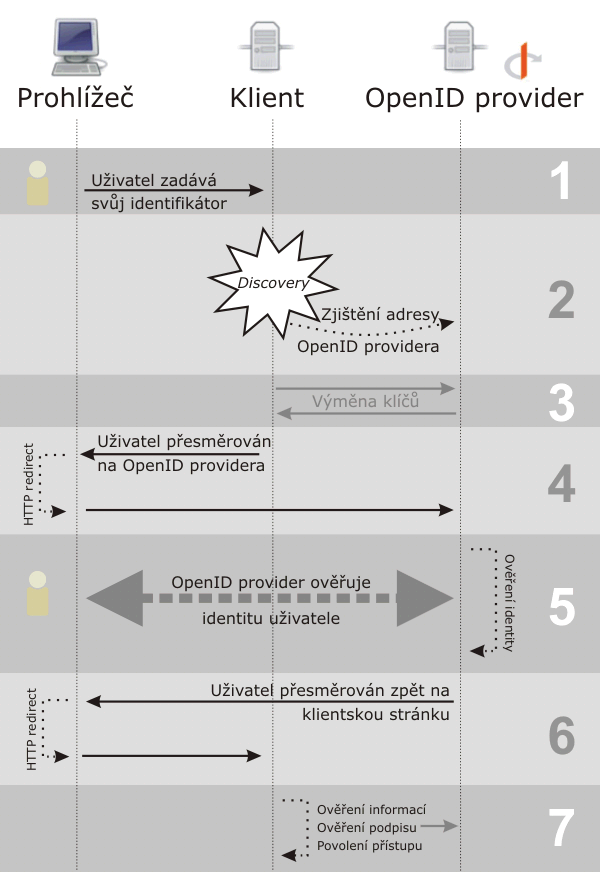
\includegraphics[width=\textwidth, keepaspectratio]{fig/openid}
	\caption{Přehled kroků probíhajících při autentizaci pomocí OpenID.
	Schéma se svolením přejato z~\cite{openid}.}
	\label{obrOpenId}
\end{figure}

Díky tomu, že si aplikace může po registrátorovi vyžádat některá
základní data o~uživateli, lze na jednoduchých službách zcela
vypustit registraci (neboli provozovat tzv. {\it tichou} registraci
při prvním přihlášní uživatele), což je pro návštěvníky nadmíru
pohodlné. Přesně této skutečnosti jsem využil i na popisovaném
projektu. Minimum nej\-důležitějších informací aplikace získá z~OpenID
identity a doplňkové údaje si potom uživatel může sám vyplnit
dodatečně v~nastavení svého účtu.

\section{Import a export dat}\label{importExport}
Jak bylo zmíněno v~úvodu kapitoly, přenosné GPS systémy se stávají
mezi běžnými lidmi stále populárnější. Jejich příznivější ceny
způsobují, že je v~dnešní době vlastní již nejeden běžec či cyklista.
Možnost importu a exportu zaznamenané trasy by tedy měla být spíše
jednou z~hlavních než doplňkových funkcí výsledné aplikace. Při
jejich implementaci jsme navíc už jen krok od interoperability
s~geografickými aplikacemi jako Google Earth nebo Google Maps. Ty
podporují buď přímo formát přenosných GPS zařízení, nebo vyžadují
svůj, který je ale rovněž založen na XML (viz \ref{xml}).

\subsection{GPS eXchange Format}
GPS navigace většinou operují v~rámci svých vlastních, uzavřených
formátů. Naštěstí se v~oblasti těch ručně přenosných vytvořil de
facto standard v~podobě GPX, formátu velmi rozšířeného výrobce GPS
navigací, společnosti Garmin. GPX je aplikací univerzálního jazyka
XML a jeho schémata jsou veřejně dostupná\footnote{Viz
\url{http://www.topografix.com/gpx/1/1/}.}.

Na formátu lze poznat zaměření pro navigace. Podporuje například
zaznamenání trasy i přes výpadky v~signálu apod.

\subsection{Keyhole Markup Language}
Společnost Keyhole, která vytvořila formát KML, již dnes přežívá
právě jen v~jeho názvu. Tvůrce programu, jenž dnes známe pod jménem
Google Earth, pohltil vyhledávací gigant již v~roce
2004\footnote{Podrobnosti dostupné na
\url{http://www.google.com/press/pressrel/keyhole.html}.}, tři roky od
jeho založení.

KML je stejně jako GPX aplikací jazyka XML a stalo se vedle něj
druhým používaným a uznávaným standardem pro záznam geografických
dat. Existuje i jeho komprimovaná verze pod názvem KMZ. Trasu
exportovanou do KML lze zobrazit nejen v~programu Google Earth, ale
také online na Google Maps, což je funkčnost poněkud revoluční. Pokud
totiž na Google Maps takovýmto způsobem napojíme online generovaná
KML, lze vytvářet dy\-na\-mic\-ky aktualizované uživatelské
mapy\footnote{Malá ukázka je k~dispozici např. ve formě zobrazení tras Tour de France
2005 --
\url{http://maps.google.com/maps?q=http://kml.lover.googlepages.com/leTourDeFrance2005.kmz&t=k}.}.
Přitom ke spojení stačí zadat adresu KML či KMZ souboru do vyhledávacího pole online map.

Generovat KML opět není nijak obtížné. Formát je otevřený a nabízí na
webu ucelenou dokumentaci\footnote{Viz
\url{http://code.google.com/intl/cs/apis/kml/}.}.

Formát KML je velmi ovlivněn tím, že vychází z~aplikace Google Earth
a obsahuje velké množství elementů i jen pro definici zobrazení
geografických dat v~aplikaci (např. zda má být nabídka v~menu
rozvinutá či svinutá). Tyto elementy však není nevyhnutelně nutné
používat.

\section{Mikroformáty}\label{microformats}
Mikroformáty jsou způsob, jak do webových stránek vkládat strojově
čitelnou informaci a přitom zůstat v~rámci syntaxe na možnostech
existujících HTML značek a atributů. Dají se tedy pochopit také jako
cesta, jak vytvořit aplikační rozhraní přímo v~HTML kódu bez
speciálních exportů do jiných formátů jako JSON nebo XML (viz
\ref{api}). Automatické nástroje (ať už klientského či robotického
charakteru) totiž potom mohou podle určitých pravidel přes DOM (viz
\ref{dom}) přistoupit k~hodnotám jednotlivých položek
mikroformátu a pracovat s~nimi.

Mikroformáty se postupně rozšiřují a získávají si oblibu i přesto, že
zatím neexistuje příliš klientských nástrojů ani mashupů s~jejich
podporou. S~přibývajícím výskytem sémanticky vyznačeného kódu
u~poskytovatelů dat lze však očekávat, že se brzy objeví. Ukázku
mikroformátů v~akci lze koneckonců spatřit i na webu
fakulty, např. u~stránky s~profilem vedoucího této práce
\url{http://www.fit.vutbr.cz/~hruska/}.

Velmi aktivně se o~technologie mikroformátů v~České republice zajímá
Martin Hassman \cite{mfLupa}. Komplexní seriál o~problematice vyšel
na serveru Zdroják.cz Janu Sládkovi \cite{mf}.

\chapter{Specifikace požadavků a rámcový návrh řešení}

Jak jsem již pro osvětlení zmínil v~úvodu práce, evidencí
geografických tras uživatele se rozumí webová aplikace, umožňující
člověku pohodlně a interaktivně zaznačit do mapových podkladů trasu,
kterou plánuje absolvovat či kterou již absolvoval například na kole,
pěšky, na bruslích nebo během. Nic samozřejmě uživateli nebrání
evidovat i jiné, delší trasy, systém by měl být však primárně určen
pro výše naznačené lokální sportovní využití.

\section{Základní koncepce}
Aplikaci jsem koncipoval jako službu, kam se uživatel zaregistruje a
potom, přihlášen na svůj účet, může zakládat trasy svých výletů. Ty má
možnost ukládat a zpětně prohlížet. Trasy jako takové neposkytují jen
interaktivní záznam cesty na mapovém podkladu, ale také statistiky a
běžné informace o~trase. Zde je prostor pro kombinaci s~dalšími
podklady –- například s~informacemi o~nadmořské výšce terénu lze
uživateli poskytnout navíc výškový profil jeho trasy. Uživatel má
možnost trasy i plánovat. V~tomto režimu aplikace vykazuje statistiky
trasy a může využít zase jiných datových zdrojů, aby poskytla lepší
obraz o~tom, co může například běžce na trase potkat (to může být
opět výškový profil, ale také např. předpověď počasí pro místo trasy
nebo vrstva s~fotografiemi místních zajímavostí či panoramat).

\section{Cílení projektu}
Cílovou skupinou projektu jsou běžci, pěší turisté, cyklisté,
běžkaři, bruslaři, jezdci na koních a třeba i vodáci. Je tedy
důležité si uvědomit, že projekt pracuje s~uživatelem, jenž nemusí
být nijak technicky vzdělán, takže by mu měl nabídnout srozumitelné a
příjemné uživatelské prostředí. Během výběru mapových podkladů (viz
\ref{vybermap}) však také vyvstává otázka, zda projekt cílit pouze na
Českou republiku, nebo počítat s~uživatelskou základnou z~celého světa.

Cílit mapový projekt celosvětově totiž neznamená jen lokalizovat
systém přinej\-menším i do angličtiny, ale také mít k~dispozici dobré
globální mapové podklady a s~nimi samozřejmě také všechna použitá
API. Území Česka a Slovenska má jednu z~nej\-dokonalejších a nej\-hustších
sítí turistického značení pro pěší turistiku \cite{kct}.
Podobné značení má také Polsko, ale jinak je takováto síť prakticky světově unikátní. To
znamená pro mou aplikaci především skutečnost, že pokud chce
poskytovat možnost zobrazení těchto tras, musí využít lokálního
poskytovatele mapových podkladů. Na druhou stranu bude potom
funkčnost systému omezena prakticky na jeden stát, protože kvalitní a
podrobné mapové podklady místních poskytovatelů nejsou v~zásadě
celosvětové.

Nabízí se dvě možnosti -- zda se vydat cestou horších podkladů, ale
oslovením větší uživatelské základny, nebo zkusit oslovit maximum
uživatelů na domácím trhu a moci odrážet jeho lokální specifika. Dá se
říci, že Češi jsou pro výše zmíněnou turistickou činnost dosti
zapálení \cite{turistika} a proto lze očekávat, že hustota
potencionálních uživatelů systému by zde byla mnohem vyšší než
v~jiných zemích, i přes zdánlivě malý, desetimilionový trh.

Specifika českého turismu, existence celosvětově operujících
konkurenčních projektů jako např. MapMyRun.com a absence vážné
konkurence na domácím trhu mě přivedla k~rozhodnutí cílit aplikaci
pouze na Českou republiku. Jak se lze dočíst v~\ref{vybranamapa},
využívám tedy nakonec podkladů lokálního poskytovatele. Navíc jsou
často na ČR omezeny i jiné zdroje dat a celý systém je pouze
v~češtině.

\section{Výběr mapového API}\label{vybranamapa}
Z~charakteru aplikace, jež je předmětem této práce, celkem jasně
vyplývá, že výběr mapových podkladů je jedním z~nej\-důležitějších
rozhodnutí, které bude mít vliv na celý další vývoj projektu.
Soustředil jsem se proto opravdu pečlivě na vlastnosti
jednotlivých API a dlouze zvažoval.

Vzhledem k~faktům zmíněným v~předcházejících odstavcích jsem však
postupně nabyl dojmu, že ani jedno řešení rozhodně nelze favorizovat a
spíše bude nutné vybrat nej\-méně bolestivý kompromis. Vybíral jsem
podle třech hlavních kritérií:
\begin{itemize}
	\item Možnosti a funkce API,
	\item kvalita mapových podkladů s~důrazem na turistické
	mapy a možnosti zobrazovat české turistické značky a cyklistické
	trasy,
	\item zázemí poskytovatele a budoucnost API.
\end{itemize}

Google nabízí bezkonkurenční API a dokonce v~současné době
představuje jeho zcela novou verzi, ale jeho mapové podklady jsou pro turistiku
v~českých podmínkách naprosto nedostatečné. Mapy.cz naopak disponují
vynikajícími mapovými podklady, jenomže jejich aplikační rozhraní je
velmi chabé z~hlediska funkcionality a ještě mnohem více omezující
v~oblasti licenčních podmínek jeho použití. Seznam.cz sice vyvíjí nové
API, ale to je zatím velmi nestabilní a jeho licence je stále
neznámá. Pro svou práci jsem tedy nakonec vybral podklady od Centrum
Holdings, protože poskytují dobré turistické mapy a mají bohatou
škálu funkcí. S~faktem, že vývoj aplikačního rozhraní je již několik
let zcela mrtvý a jeho budoucnost je nejistá, mi nezbylo než se
smířit a počítat s~tím, že v~budoucnu ji možná bude zapotřebí přepsat
pro jiné API. V~tomto ohledu bych vzhlížel k~vývoji nového API v~Seznam.cz.

\section{Nástroje pro výškový profil}
Pro svůj projekt jsem se rozhodl použít jako primární zdroj dat
Výškopis.cz a v~podobě záložního jsem implementoval API s~méně
přesnými výsledky od GeoNames.org. Výškopis.cz má také výhodu
přítomnosti metody pro získání série dat v~jednom požadavku. Ta je
důležitá -- velmi usnadňuje řešení situací, kdy aplikace potřebuje
v~jednom okamžiku zjistit nadmořskou výšku z~celé řady míst na mapě.
Takový problém se běžně nedá řešit sérií samostatných požadavků na
server s~API, protože ten je tak nárazově zatížen a nestíhá na
požadavky odpovídat.

Zvážil jsem, že pro vykreslení grafu by knihovny zřejmě dokázaly
poskytnout sofistikovanější výstup, ale hledal jsem spíše rychlé a
jednoduché řešení a tím se ukázalo být Google Chart API. V~případě,
že by v~budoucnu svými základními funkcemi nedostačovalo, je zde vždy
možnost nahradit jej jednou z~výše zmíněných knihoven.

\section{Výběr ostatních služeb}
V~oblasti ostatních podkladů není příliš velký prostor
k~závěrečné rozvaze a následnému výběru. Už prvotní analýza totiž při
nich dospěla k~závěru, že služby jsou buď poskytovány pouze jedním
serverem, nebo je nelze vůbec zahrnout.

\section{Výpočet statistik}
K~výpočtu statistik uživatelských výkonů a specifik tras stačí
využití běžné matematiky a všeobecně známých fyzikálních vzorců. Pro
zpřesnění je nutné si dohledat termíny jako např. převýšení (součet
všech rozdílů nadmořských výšek na úsecích trati, kde sportovec stoupá) nebo
členitost terénu (dána rozdílem nej\-níže položeného a nej\-výše
položeného místa v~oblasti), ale i ty jsou celkem obecně známé.

Jedinou specialitou je výpočet energie spotřebované na trati. Ten se
odvíjí od tabulkových hodnot v~$kJ / kg \cdot min$ závisejících na
hmostnosti, rychlosti, doby výkonu a typu činnosti. Z~různých
internetových zdrojů jsem tyto hodnoty sesbíral a utřídil do tabulky,
kterou jsem uložil do databáze jako persistentní data.

\section{Export a import dat}
Z~hlediska interoperability se jeví implementace pro výměnu
dat s~přenosným GPS zařízením nebo aplikací Google Earth jako
klíčová. Vlastnost jsem tedy považoval spíše za nutnou než volitelnou.

U~každé trasy je možnost vyexportovat si ji do GPX nebo KML (viz
\ref{importExport}). Pro popularizaci možností formátu KML ve spolupráci s~online mapami jsem
přidal i třetí volbu -- možnost otevřít trasu v~Google Maps. V~obou
formátech lze také trasu přímo importovat do aplikace jako novou trasu
namísto jejího ručního klikání do mapy.

\section{Způsob autentizace}
Výhoda OpenID (viz \ref{openid}), tedy jednoznačná identifikace uživatele
napříč webem, je i jeho hlavní nevýhodou. Uživatelé nejsou zvyklí na webu
vystupovat pod svým jménem nebo jinak jednoznačně identifikovatelní a
často jim právě z~hlediska určité anonymity diverzita účtů i vyhovuje.

I~vzhledem k~současné podpoře OpenID je vše teprve v~začátcích a
povědomí o~službě není tak velké. Mohlo by být tedy celkem rizikové
metodu nasadit jako jediný způsob registrace a přihlášení do aplikace.
Protože ale OpenID nasadil i hegemon českého internetu
Seznam.cz\footnote{Nápověda
k~OpenID je na \url{http://napoveda.seznam.cz/cz/login/openid/}.},
u~něhož většina Čechů účet má, rozhodl jsem se tuto nej\-pokrokovější metodu
autentizace implementovat opravdu bez alternativy. Získání
OpenID od Seznam.cz je navíc velmi snadné -- stačí ve své e-mailové
adrese (např. {\tt uzivatel@seznam.cz}) zaměnit znak zavináče za
písmena {\tt id} oddělená tečkami ({\tt uzivatel.id.seznam.cz}).

Rozhodnutí implementovat OpenID bez alternativy je nutné přehodnotit
až po nějaké době existence aplikace a zpětné vazbě
stávajících, ale i potencionálních uživatelů. Pokud by OpenID
bylo pro službu spíše handicapem než přínosem, je systém navržen tak,
že lze snadno i se zachováním podpory pro OpenID doprogramovat druhý
způsob přihlašování a samostatnou registraci.

\section{Využití mikrofotmátů}
Při tvorbě práce zřejmě mikroformáty (viz \ref{microformats}) nebude možné
příliš využít. Množiny specifikovaných mikroformátů a prvků stránek použitých
v~projektu se totiž příliš neprotínají. Na několika místech by šlo
implementovat například
hCard\footnote{Viz
specifikace \url{http://microformats.org/wiki/hcard}.} –- pro
vyznačení adresy uživatele (výchozí lokace na mapě) nebo
provozovatele služby. Z~ostatních mikroformátů je zajímavý především
geo\footnote{Viz specifikace
\url{http://microformats.org/wiki/geo}.}, který specifikuje zaznačení
zeměpisných souřadnic do webové stránky. Nachází se však zatím
v~rozpracovaném stavu a je označen jako koncept\footnote{Tato
skutečnost ale například nijak nebránila vyhledávači Seznam.cz přidat
pro něj podporu \cite{geoSeznam}.}.

\chapter{Použité technologie}\label{technologie}
Množina technologií použitých na tomto projektu by se dala označit
v~rámci webového kontextu za vyloženě tradiční. Experimentům s~ne tak
rozšířenými technologiemi brání v~rámci malých projektů špatná
dostupnost jiných hostingových služeb, než těch pro jazyk PHP (viz
\ref{php}). Lze samozřejmě připravit vlastní instalaci serveru nebo
využít služeb specializovaných hostingových programů, ale to by pro aplikaci do
budoucna znamenalo velmi omezenou přenosnost a udržovatelnost. Pro
použití tradičních webových jazyků také hovoří existence mnoha
hotových řešení, podpůrných knihoven a podpory nástrojů a návodů.

V~oblasti uživatelského rozhraní navíc ani velký prostor pro výběr
není. Dá se sice uvažovat o~použití technologií jako Adobe Flash, Microsoft
Silverlight apod., ale ty vyžadují zásuvné moduly na straně klienta
a to velmi omezuje jejich přístupnost. Lze namítat, že ani jazyk
JavaScript není podporován mnoha zařízeními, je ovšem alespoň
standardem nezávislým na operačním systému a podporovaném napříč všemi
moderními prohlížeči. V~poslední době jej začínají implementovat i
nej\-novější mobilní zařízení.

V~mnoha případech jsem využil výhod frameworků, tedy komplexů
knihoven řešících rutinní problémy v~daných jazycích a usnadňující
programátorovu práci. Ten se může soustředit na řešení samotného
problému, místo aby se většinu času zabýval \uv{vynalézáním kola}.

Ke konci kapitoly se zabývám použitím technologií souvisejících s~API
jako architekturou REST nebo formáty XML a JSON.

\section{Uživatelské rozhraní webové stránky}\label{gui}
Uživatelské rozhraní, tedy GUI ({\it Graphical User Interface}),
webových aplikací je tvořeno kombinací značkovacího jazyka, stylu a
případně skriptů. Výsledek se často mezi webovými tvůrci označuje
jako tzv. {\it šablona webu} nebo {\it kód webu}.

Značkovací jazyk je zpravidla z~rodiny HTML či XML a slouží
k~zaznamenání sémantiky dokumentu. Styl, připojovaný většinou v~podobě
externího souboru, slouží k~definici vzhledu dokumentu. Pro HTML je
to nej\-častěji CSS, zatímco v~aplikacích XML se setkáme asi spíše
s~XSL. Třetí vrstvou bývá v~moderních projektech skriptovací
jazyk, jenž se spouští na klientském prohlížeči během a po vykreslení
webové stránky. Má schopnost dynamicky měnit obsah i styl dokumentu,
v~čemž mu pomáhá úzká spolupráce s~technologií DOM. Takovým skriptovacím
jazykem je dnes již prakticky pouze JavaScript, jemuž se za svou
existenci podařilo dospět do široce podporovaného jazyka a který
z~webu vytlačil všechny své potencionální konkurenty (např. VBScript
společnosti Microsoft).

\subsection{Sémantický dokument s~HTML}
HTML\footnote{Specifikace: \url{http://www.w3.org/TR/html401/}.}
({\it HyperText Markup Language}) je jazyk pro snadné značkování dokumentů a
jejich šíření po webu přes protokol HTTP. Tim
Berners-Lee jej spolu s~tímto protokolem v~roce 1990 sestavil, aby
pro svět objevil technologii webu. HTML je aplikací SGML ({\it
Standard Generalized Markup Language}), univerzálního jazyka pro značkování
dokumentů\footnote{HTML se aplikací SGML stalo ve verzi 2.0 a od
připravované verze 5 se opět od tohoto vztahu upouští.}.
\cite{htmlHistory}

HTML disponuje množinou elementů, jež je možné použít k~značkování
dokumentu (např. {\tt <p>Text odstavce</p>}). To má za výsledek
přiřazování významu částem textu a možnost odlišení jejich zpracování
či zobrazení. Bohužel sémantická vybavenost HTML již příliš
nepostačuje dnešním potřebám a proto se můžeme setkat s~aktivitami
jako např. mikroformáty (viz \ref{microformats}) nebo snahami
o~posílení sémantiky v~právě připravované verzi, HTML5 \cite{html5}.

Značky v~rámci zápisu dokumentu tvoří stromovou strukturu. Této
skutečnosti využívá technologie DOM (viz \ref{dom}). Informaci
o~tom, kde může být jaký element a co může obsahovat se nachází
v~tzv. DTD ({\it Document Type Definition}), připojovaném na samý
začátek HTML dokumentu. Jazyk HTML má DTD už připravená k~použití
(např. \url{http://www.w3.org/TR/html4/strict.dtd}) a připojují se
prakticky bezvýhradně externím odkazem. Nejen v~závislosti na
použitém typu DTD prohlížeče často mění zpracování šablony dokumentu,
především jejích stylů. DTD lze použít i pro XML, ale pro něj je lepší
použít sofistikovanější nástroje jako např. XML Schema. 

\subsection{Výběr HTML místo XHTML}
O~vývoj jazyka HTML a souvisejících webových standardů se stará
sdružení internetových firem, výrobců prohlížečů a jiných
zainteresovaných subjektů, W3C ({\it World Wide Web Consortium}). Po
uvedení velmi úspěšného formátu XML přišla tato organizace
s~myšlenkou transformovat HTML na aplikaci tohoto univerzálního
značkovacího jazyka. Výsledkem snah se stal jazyk
XHTML\footnote{Specifikace: \url{http://www.w3.org/TR/xhtml1/}.}, tedy
{\it Extensible Hypertext Markup Language}. S~jeho uvedením byl vývoj
\uv{starého} HTML oficiálně ukončen v~poslední verzi 4.01.

W3C poté pokračovalo ve vývoji XHTML 2.0, které mělo být navíc již
zcela nekompatibilní s~původním HTML. První verze XHTML však
nepřinesly do HTML nic nového a v~podstatě způsobovaly jen problémy
navíc \cite{xhtml}:

\begin{itemize}
	\item Špatná podpora správného MIME typu XHTML {\tt
	application/xhtml+xml} ze strany nej\-rozšířenějšího prohlížeče,
	Internet Exploreru, nasazení \uv{opravdového} XHTML v~praxi zcela
	znemožňovala.
	\item Počet elementů zůstal oproti HTML de facto nezměněn.
	\item Syntaktická striktnost parseru XHTML po vzoru XML sice
	nedovolovala vývojáři dělat chyby, ale ty bohužel v~praxi nevznikají
	jen jeho přičiněním. Nekorektnost zápisu přitom způsobovala ukončení
	zpracování dokumentu a nedostupnost jeho obsahu.
	\item Rozšiřitelnost, hlavní lákadlo XHTML (viz jeho název), nebylo
	v~praxi příliš využíváno. 
\end{itemize}

Vývoj standardu XHTML 2.0 ve W3C později navíc téměř ustrnul. Když
webdesignerská obec objevila problémy XHTML a pochopila, že cesta
k~XML byla slepá, začala vznikat iniciativa WHATWG Iana
Hicksona. Ta oslovila tvůrce prohlížečů a začala v~konsensu s~nimi
vyvíjet novou specifikaci jazyka HTML nazývanou HTML5. Akt se setkal
s~velkým ohlasem, protože WHATWG se snaží do jazyka promítnout
požadavky dnešních vývojářů webových aplikací a řešit existující
problémy jako nepostačující sada formulářových prvků, slabá sémantika
dokumentu, značky pro audio a video aj. \cite{whatwg}

Za datum definitivní změny směru vývoje lze považovat 7. březen 2007,
kdy W3C založilo novou pracovní skupinu HTML, v~níž se prakticky spojilo
s~aktivitami WHATWG, uznalo HTML5 jako budoucnost webu a vzalo
jej pod svou hlavičku. Tim Berners-Lee, v~současné době ředitel
konsorcia W3C, navíc 2. července 2009 oznámil\footnote{Viz zpráva
\url{http://www.w3.org/News/2009\#item119}.}, že vývoj XHTML2 bude
pokračovat už jen do konce roku 2009. Na základě všech těchto
skutečností jsem se rozhodl pro práci použít jazyk HTML a vyhnout se
XHTML, zjevně již neperspektivní technologii.

\subsection{Styly pomocí CSS}\label{css}
CSS\footnote{Specifikace: \url{http://www.w3.org/TR/CSS21/}.} ({\it
Cascading Style Sheets}) je jednoduchý deklarativní jazyk pro definici vzhledu
dokumentu zapsaného ve značkovacím jazyku. Lze
jej připojit jak k~HTML a XHTML, tak i k~XML. Vznikl ve
standardizační organizaci W3C za účelem pomoci očistit HTML od
prezentačních značek a navrátit jeho použití k~sémantickému
značkování dokumentů. To se v~zásadě povedlo a se stoupající podporou
v~prohlížečích tvůrci webu začali vzhled definovat většinou pouze
pomocí externích stylů. To poskytuje především několik výhod
\cite{css1}:

\begin{itemize}
	\item Styl je možné aplikovat na několik dokumentů najednou a jeho
	použitím se lze vyvarovat redundanci. HTML dokument je menší a
	rychleji se zpracovává.
	\item Změnou ve stylech dokumentu lze velmi rychle a jednoduše
	změnit třeba i celý vzhled stránky bez zásahu do vlastního HTML
	kódu.
	\item Extrahováním informace o~vzhledu do CSS dostáváme HTML zápis,
	který je čistým sémantickým značkováním textu a zpracování takového
	HTML je jednodušší. Toho využívají nejen alternativní klienti pro
	přístup k~webu, ale také např. velmi důležití vyhledávací roboti.
	\item CSS má větší možnosti formátování než původní formátovací
	značky v~HTML.
\end{itemize}

Vlastní zápis definice vzhledu v~CSS je poměrně intuitivní. Tzv. {\it
selektorem} se vybere množina elementů a na tu se poté aplikují
pravidla (např. {\tt p \{ color: red; font-size: 75\%; \}}).
Aplikování pravidel se však uplatňuje na základě složitého mechanismu
kaskády, kdy později definovaná pravidla a pravidla s~konkrétnějšími
selektory mají větší prioritu. \cite{css2}

V~současné době se dokončuje revize 2.1 tohoto jazyka. Zatímco
Internet Explorer 6, jenž má dnes i po vydání nových verzí 7 a 8
majoritní podíl na trhu, zcela neimplementuje ani CSS verze 2, jiné
moderní prohlížeče již s~předstihem zavádějí podporu pro konstrukce
navržené v~teprve připravovaném CSS3. Různost implementací podpory CSS
a jejich chyby jsou hlavní nevýhodou tohoto jazyka. Vzhledem k~vydaným
novým verzím prohlížeče Internet Explorer, jenž na dlouhodu dobu
\uv{zaspal} a vývoj zabrzdil, se však zdá, že situace se nyní již
bude rok od roku jen zlepšovat.

\subsection{Technologie DOM}\label{dom}
Objektový model dokumentu, tedy DOM\footnote{Specifikace:
\url{http://www.w3.org/DOM/DOMTR}.} ({\it Document Object Model}), je
objektová reprezentace hierarchického stromu XML nebo HTML dokumentu. DOM
funguje jako aplikační rozhraní pro přístup k~jednotlivým uzlům
dokumentu jako by se jednalo o~objekty a umožňuje číst jejich
vlastnosti, měnit je a vykonávat nad nimi funkce. Vznikl postupnou
standardizací přístupu ke zpracování XML a HTML a zavedla jej
organizace W3C. Specifikace je nezávislá jak na platformě, tak i na
implementačním jazyku.

Rozebrání dokumentu na bázi DOM vyžaduje mít jej zpracován celý a
celý jej nahrát do paměti ještě před začátkem jakékoliv manipulace.
To je výhodné, pokud k~elementům přistupujeme náhodně, ale může to
vést ke zbytečné neefektivitě aplikace, jestliže chceme dokument
zpracovat rychle a postupně. Proto vznikl i alternativní
přístup rozebrání XML, tzv. SAX ({\it Simple API for XML}).
Ten sekvenčně prochází XML a při jednotlivých událostech (začátek
elementu, konec elementu apod.) volá předdefinované metody.

Uvedení technologie DOM bylo v~oblasti uživatelského rozhraní webové
aplikace významným pokrokem. Díky jeho standardizaci se mohlo
provést např. napojení jazyka JavaScript na toto API a získat tak velmi mocný
nástroj pro manipulaci s~HTML dokumentem u~klienta.

\subsection{Skriptovací jazyk JavaScript}\label{javaScript}
JavaScript je multiplatformní skriptovací jazyk, původně vyvinutý
společností Netscape. V~prohlížeči se interpretuje během načítání a po
načtení dokumentu, k~němuž je připojen a může tak dynamicky měnit
jeho strukturu i obsah. Jeho název je čistě marketingový, s~jazykem
Java nemá nic společného a kromě podobnosti syntaxe na něj ani nijak
nenavazuje. Spolu s~aplikačním rozhraním DOM pro přístup do struktury
dokumentů HTML a XML je JavaScript silným nástrojem pro tvorbu GUI.
\cite{jsBook}

JavaScript je sice objektově založený, ne však způsobem
dědění od tříd (jak jej známe u~Javy nebo C++), ale klonováním
prototypů (tzv. {\it prototypově založené programování}, v~jehož rámci
je JavaScript zřejmě nej\-známějším představitelem). Zápis jazyka vychází,
jak již bylo naznačno stejně jako Java, z~oblíbené syntaxe jazyka C.
Dnes se používá nej\-častěji pro tvorbu dynamických uživatelských
rozhraní webových aplikací, ale svou významnou roli hraje např. i
v~XUL, formátu pro tvorbu uživatelských rozhraní desktopových
aplikací\footnote{XUL je používán především v~produktech Mozilla jako
prohlížeč Firefox nebo e-mailový klient Thunderbird. Staví na
existujících a známých technologiích jako XML, CSS, JavaScript a DOM,
čímž zpřístupňuje tvorbu GUI široké skupině vývojářů bez nutnosti
zdlouhavého studia nových metod.}.

JavaScript je dnes pod názvem ECMAScript standardizován na základě
konsensu výrobců prohlížečů, takže jeho použití již není tak
frustrující jako v~dřívějších letech, kdy byl interpretován pokaždé
jinak. I~tak se však na jeho podporu nelze spolehnout plně, protože
nejen že si jej uživatel může v~prohlížeči vypnout, ale také existuje
celá řada zařízení, jež jej vůbec nepodporují.
Z~hlediska cílení webu na běžné uživatele jsou v~tomto nej\-významnější
mobilní zařízení. I~ta ale podléhají a začínají JavaScript
implementovat (např. Apple iPhone).

\subsection{Asynchronní požadavky}\label{ajax}
AJAX je zkratkou pro {\it Asynchronous JavaScript and XML} a
představuje spíše techniku než technologii. Ač se v~jeho názvu
zmiňují konkrétní jazyky, je AJAX dnes spíše obecným označením pro
dosažení asynchronního požadavku na server z~webového uživatelského
rozhraní. \cite{ajax}

Základem AJAXu je existence objektu {\it XMLHttpRequest} (zkracováno
na XHR), jež JavaScriptu umožňuje zavolat serverový skript i mimo
klasické schéma požadavek/odpověď. Tendence asynchronní práce se
serverem zde však existovaly již dlouho před tímto objektem --
jednou z~nich je například existence elementu {\tt IFRAME} v~HTML.
Objekt XHR zavedl Microsoft v~rámci rozšíření ActiveX v~Internet
Exploreru 5. Protože však toto řešení postrádalo podporu napříč
ostatními prohlížeči, mezi vývojáři se neujalo. To se ale časem
změnilo a technku oprášil Google při tvorbě webových aplikací jako
Google Suggest, Google Maps nebo Gmail. AJAX byl roku 2005 pojmenován
v~článku J. J. Garretta \cite{ajaxArticle} a dostal se do obecného
povědomí vývojářů.

Zajímavostí je, že objekt XMLHttpRequest stále ještě není
standardizován a jeho podpora tedy závisí jen na \uv{dobré vůli}
tvůrců prohlížečů. Ti jej však až na detaily implementovali jednotně
a tak lze AJAX bez problémů používat i bez oficiální standardizace,
která jej čeká pravděpodobně v~rámci DOM.

Výhody AJAXu jsou zřejmé. Umožňuje dlouho neuskutečnitelný přenos dat
i mimo znovunačtení celé stránky, což vede ke vzniku opravdu
sofistikovaných webových aplikací, jež mají velmi podobné vlastnosti
jako aplikace desktopové. Tím, že přenáší jen data, která potřebuje,
stránka navíc snižuje provoz na serveru (na druhou stranu zase
zvyšuje počet HTTP požadavků). Nevýhody plynou především ze změny
paradigmatu používání webu. Uživatel například změnu na stránce
nemusí vůbec zpozorovat nebo se na takovou stránku nemůže odkázat
pomocí jedinečného URI. Existují již však návrhové vzory, které tyto
problémy řeší.

AJAXová aplikace si ze serveru asynchronně žádá data a ta dostává
zpravidla ve třech možných formách. Buďto jako obyčejnou textovou
informaci (to se hodí, pokud očekává např. jediné číslo, jediný
řetězec, úsek HTML kódu apod.), XML, nebo JSON (viz \ref{xml} a
\ref{json}).

\subsection{Framework MooTools}
Ke zjednodušení rutinní práce s~JavaScriptem a odstínění rozdílů
v~jeho implementaci je užitečné používat nějaký framework. Bez takové sady
knihoven se dnes neobejde žádná z~velkých internetových společností --
konkrétně například Google a Wikipedia nej\-častěji využívají jQuery,
Microsoft MooTools, Yahoo! má svůj vlastní framework. Mezi známými projekty jako
Prototype či již zmíněnými jQuery a MooTools jsem nakonec vybral
poslední zmíněný.

Prototype a MooTools jsou architekturou založené na rozšiřování
existujících objektů JavaScriptu, čímž dosahují poměrně
efektivních konstrukcí. Na druhou stranu zasahují do jádra
jazyka a mění jej, takže způsobují nekompatibilitu s~jinými nástroji.
V~tomto ohledu je možná lepší druhý přístup, který prosazuje jQuery, a
to izolovat všechny funkce frameworku do samostatného jmenného
prostoru a zabránit tak jakýmkoliv kolizím. Knihovna jQuery se tedy
zdála lepší volbou, nicméně API mapových podkladů, jež jsem vybral
(viz \ref{vybranamapa}), již obsahovalo MooTools a proto jsem toho
bez většího rozhodování využil a nastudoval tento framework. I~přes
všechny různé vlastnosti jsou totiž přední JavaScriptové frameworky
srovnatelné a základní metody pro práci s~DOM, tvorbu jednoduchých
efektů, usnadnění práce s~AJAXem aj. poskytují všechny.

Jedním z~podstatných ulehčení je na JavaScriptových frameworcích,
MooTools nevyjímaje, systém přístupu k~elementům v~HTML dokumentu.
Autoři frameworků se nechali inspirovat selektory v~CSS (viz
\ref{css}) a zavedli pro ně podporu i v~rámci JavaScriptu. Pokud tedy víme, jak bychom
k~danému prvku stránky přistoupili pomocí stylů, můžeme stejný zápis
předat speciální metodě frameworku a ta nám na jeho základě přes DOM
vrátí objekt požadovaného elementu, s~nímž lze dále pracovat. To je
samozřejmě pro webové tvůrce velmi efektivní, protože to nejen usnadňuje velmi rutinní
záležitost a odstiňuje práci se samotným DOM, ale také recykluje
znalosti, které má programátor již ze psaní stylů.

MooTools jsou, stejně jako jiné současné JavaScriptové frameworky,
testovány na všech majoritních prohlížečích zahrnujících i Internet
Explorer 6.

\section{Serverová část}\label{mvc}
Část aplikace nacházející se na serveru má za úkol perzistentně
ukládat data a zpřístupňovat je, dynamicky generovat uživatelské
rozhraní a poskytnout logiku, která bude řídit pochody v~aplikaci
v~závislosti na požadavcích ze strany uživatele. Zmíněné tři funkce se
dají interpretovat také jako tři vrstvy známé softwarové architektury
MVC, tedy {\it Model-View-Controller} (kde písmenům zmíněné funkce
odpovídají přesně podle uvedeného pořadí). \cite{janTichy}

Jak jsem již zmínil v~\ref{technologie}, výběr serverového
programovacího jazyka, jenž by byl jádrem aplikace, byl z~důvodu
dostupnosti hostingových služeb a budoucnosti projektu omezený. PHP
(viz \ref{php}) splňovalo všechny požadavky, ve svých nových verzích
nabízí plnohodnotný objektový přístup a existují pro něj velmi dobré
frameworky. Z~těch jsem použil relativně nový český framework Nette
(viz \ref{nette}), který plně využívá objektového PHP a je
architekturou spřízněn s~výše zmíněným vzorem MVC.

Jako úložiště perzistentních dat jsem využil relační databázi. Kvůli
podobným omezením hostingového trhu jako u~jazyka PHP jsem ani zde
neměl příliš perspektivních možností k~výběru a jako systém
řízení báze dat jsem použil MySQL.

\subsection{Jazyk PHP}\label{php}
PHP (rekurzivní zkratka {\it PHP: Hypertext Preprocessor}) je
interpretovaný skriptovací jazyk nezávislý na platformě, přímo
vytvořený pro tvorbu dynamicky generovaných webových stránek. Jeho
vznik sahá až k~roku 1994. Syntaxí navazuje na jazyk C, ale celkově
vychází spíše z~Perlu. Má velmi rozsáhlou sadu knihoven dostupných
již ze základní instalace (jmenujme alespoň vestavěnou podporu pro
většinu databázových systémů, řadu internetových protokolů, nástroje
pro práci s~XML a mnoho dalšího). PHP se stalo pravděpodobně
nej\-oblíbenějším jazykem pro dynamické generování webových
stránek\footnote{Viz \url{http://www.php.net/usage.php}.}. Je na něm
postaveno mnoho známých projektů jako encyklopedie Wikipedia,
redakční systém WordPress, fórum phpBB a další. \cite{phpBook}

Nevýhodami PHP mohou být mírně nekonzistentní vývoj a formát funkcí,
nemožnost udržet kontext aplikace (při každém požadavku se vlastně
celá aplikace spouští znova), nesnadné lazení aplikací, špatná
podpora Unicode a chybějící jmenné prostory. Poslední dva jmenované
problémy má řešit připravovaná verze 6.

Pomocí PHP se na straně serveru dle požadavků
uživatele dynamicky generuje HTML kód. Ten se následně pošle na
výstup jako každá jiná statická stránka a klient je tedy od
samotného PHP izolován a do styku přichází jen s~jeho produktem,
uživatelským rozhraním (popsáno v~\ref{gui}). Abych byl přesný,
výstupem skriptu samozřejmě nemusí být pouze HTML. V~PHP lze
pružně vytvořit cokoliv -- XML v~podobě RSS, ale třeba i
obrázek nebo PDF.

\subsection{Systém řízení báze dat MySQL}\label{mysql}
Multiplatformní relační databázový systém {\it MySQL} je opět zřejmě
nej\-oblíbenější a běžně nej\-dostupnější variantou nástroje svého druhu. Systém
vyvinula švédská firma MySQL~AB. Ta se nej\-dříve stala
akvizicí společnosti Sun, aby před nedávnem došlo ke spojení ještě
většímu a oba zmíněné subjekty začne v~blízké době vlastnit databázový
gigant Oracle. Jelikož je MySQL možnou konkurencí Oracle, není budoucnost
této databáze jasná \cite{mysql}. Systému MySQL využívá mnoho známých produktů psaných v~PHP (viz
\ref{php}), ale také velké společnosti jako např. Google.

MySQL byla i se svým dialektem jazyka SQL od začátku vyvíjena jako
lehká a rychlá databáze \cite{sql}. Proto byly některé (mohlo by se
zdát zásadní) funkce přidávány až v~posledních letech, kdy začaly chybět vývojářům
stavějící na MySQL své aplikace. Od verze 5 (od roku 2005) však
podporuje již většinu svých kritizovaných nedostatků.

Často se při vývoji webových aplikací používá pro přístup k~databázi
mezivrstva, jež abstrahuje rozdíly jednotlivých SŘBD a umožňuje tak
programátorovi kdykoliv v~budoucnu správu perzistentního úložiště
vyměnit. Taková vrstva je použita i v~mé práci, která je v~důsledku
toho na druhu SŘBD závislá minimálně. Vrstva se jmenuje {\it dibi},
je naprogramovaná v~PHP a jedná se o~projekt úzce spjatý s~Nette
Frameworkem (viz \ref{nette}).

\subsection{Nette Framework}\label{nette}
Programování v~PHP samotném je na abstraktnější úrovni než např.
vývoj v~jazyce C, ale i tak není možné vyhnout se rutinním a
problémovým konstrukcím, které je třeba stále znova řešit. U~webových
aplikací, které v~podstatě vycházejí všechny ze stejných principů a
postupů, to platí v~ještě větší míře. Řešením je použít framework.

{\it Nette Framework} je open-source\footnote{Od roku 2008. Framework
podle slov jeho autora a hlavního vývojáře Davida Grudla existuje již od
roku 2004.} knihovna napsaná v~čistě objektovém PHP5. Je tak
pokroková, že využívá dokonce nej\-novější verze PHP5.3 z~30. června
2009\footnote{Existují samozřejmě souběžné verze frameworku i pro
starší PHP.}. Nette je sestaveno z~modulů, které lze často použít i
samostatně, nezávisle na sobě. Tímto rysem se podobá rozsáhlému
frameworku Zend od tvůrců PHP. Na rozdíl od něj je však mnohem menší
a i výkonnější \cite{netteTest} \cite{netteCo}.

Nette vychází pod derivátem BSD licence a lze na něm proto stavět
komerční aplikace. Vyrostla kolem něj aktivní komunita vývojářů a brzy
na něm začaly programovat weby i velké tuzemské společnosti. Jmenujme
např. Mladou Frontu nebo Internet Info (vydavatel Lupa.cz, Root.cz).

Přednostmi Nette Frameworku je jeho česká podpora,
pokrokovost, inovativní myšlenky, efektivní integrovaný šablonovací
systém, výkonnost, zabudované ladící nástroje a také modulárnost,
která jej umožňuje kombinovat s~jinými knihovnami. Z~hlediska
architektury je Nette založeno na upraveném vzoru MVC (viz \ref{mvc})
a funguje na bázi událostmi řízeného návrhu. Jedním z~důležitých aspektů je také
rychlý vývoj frameworku. Nette je stále poměrně nové, ale komunita
kolem něj za poměrně krátkou dobu vytvořila již poměrně rozsáhlou
dokumentaci\footnote{Viz \url{http://nettephp.com/cs/dokumentace}.}.
\cite{netteProc}

\section{Práce s~API}\label{api}
API služeb relevantních pro tento projekt je poskytováno v~zásadě
dvěma způsoby. Dodavatelé se většinou vyhýbají složitým protokolům či
technologiím a nabízejí jednoduchá a přístupná aplikační rozhraní.
Funkčnost API tak lze získat buď přímo pomocí vzdálených souborů
s~kódem v~jazyce JavaScript (viz \ref{javaScript}), nebo, pokud služba
nabízí data přímo, pomocí rozhraní REST ({\it Representational State
Transfer}, \ref{rest}).

\subsection{Vzdálené volání skriptů}
Skripty připojujeme jako běžně v~hlavičce či těle HTML
dokumentu, akorát využíváme vzdálených souborů namísto lokálních.
Vzdálené soubory se skripty jsou většinou vázány na tzv. {\it API
klíč}, který je zapotřebí vygenerovat zpravidla pro doménu, na níž má
probíhat provoz aplikace. Při použití na jiném serveru potom API
nefunguje a je potřeba vygenerovat nový klíč. Poskytovatelé díky tomu
mohou kontrolovat dodržování podmínek použití API, např. limity
požadavků aj. Kontrola klíče je často inteligentní a není aplikována
při použití na vlastním stroji (IP adresa 127.0.0.1, tzv. {\it
localhost}) za účely vývoje a ladění aplikace. Zajímavá možnost je
připojovat a odpojovat skripty k~dokumentu dynamicky, pomocí jiného
řídícího skriptu a technologie DOM (viz \ref{dom}).

\subsection{Technologie REST}\label{rest}
REST je architektura představená v~roce 2000 jedním z~autorů
specifikace protokolu HTTP \cite{rest}. Pro naše účely by API
v~podobě REST šlo ve zkratce popsat jako technologii, v~níž poskytovatel dat
zveřejní webové URI, MIME typ odpovědi a množinu operací, které jsou k~dispozici
přes HTTP metody POST, GET, PUT nebo DELETE. V~praxi
potom máme například adresu {\tt \url{ws.geonames.org/gtopo30JSON}},
víme z~dokumentace GeoNames.org, že můžeme použít parametry {\tt lat} a {\tt
lng} pro určení souřadnic a že výsledkem bude JSON s~nadmořskou
výškou. Když tedy vytvoříme požadavek na adresu
{\tt \url{http://ws.geonames.org/gtopo30JSON?lat=47.01&lng=10.2}},
dostaneme přes HTTP patřičnou odpověď ve formátu JSON.

Z~formátů odpovědí jsou nej\-využívanější obyčejný text, XML (\ref{xml})
a JSON (\ref{json}). Vyjímečně se lze také u~specifických služeb
setkat s~jinými, jako např. u~Google Chart API, kde lze přes REST
pohodlně vygenerovat obrázek s~grafem (použití v~\ref{grafy}).

\subsection{Univerzální jazyk XML}\label{xml}
XML, celým názvem {\it Extensible Markup Language}, je obecný
značkovací jazyk. Byl vytvořen se záměrem poskytnout univerzální
řešení pro značkování dat a dokumentů. XML vlastně ani není kompletní
deklarativní jazyk, protože neobsahuje sémantiku. Značky XML jsou
prakticky totožné se značkami jak je známe z~HTML, jen jejich názvy
nejsou předem určeny. Můžeme si díky tomu v~rámci XML vytvořit skupinu
vlastních pravidel a názvů (pomocí popisů jako DTD nebo např. XML
Schema). Takovým vymezením konkrétních značek zavádíme do XML sémantiku a
získáme tzv. {\it aplikaci XML}, tedy jeho podmnožinu pro konkrétní
použití.

Aplikacemi XML jsou např. formát pro syndikaci publikovaných článků
RSS, formát pro vektorovou grafiku SVG, publikační nástroj DocBook,
protokol XMPP (znám jako {\it Jabber}), ale např. i nej\-novější
formáty kancelářských balíků jako Office Open XML a OpenDocument.

XML jako nosič dat lze v~aplikacích snadno zpracovávat a díky jeho
rozšířenosti jsou pro to nástroje do programovacích jazyků zabudovány
již často v~základní výbavě. Dva základní přístupy ke
zpracování XML jsou DOM a SAX (oba popsány v~\ref{dom}). Jednou
z~možností jak zpracovávat XML je navíc jeho transformace do jiného typu
dokumentu (např. do HTML, PDF) pomocí stylů XSL.

Všechny tyto vlastnosti dělají XML velmi výhodným jazykem pro přenos
a uchování strukturovaných textových informací. XML má však i své
nevýhody a ty lze vidět především u~minimalistického použití jako
v~případě AJAXu nebo různých API (viz \ref{ajax} a \ref{rest}). Pokud
chceme pomocí XML doručovat jednoduché struktury a základní datové typy, zjistíme, že systém
tohoto jazyka je pro naše účely příliš komplexní a jeho fragmenty
nesou více informací v~názvech značek než mezi nimi. Proto vznikly
tzv. \uv{odlehčené}, lidsky čitelné formáty jako YAML nebo JSON.

\subsection{Lidsky čitelný JSON}\label{json}
Jak napovídá celý název, {\it JavaScript Object Notation}, JSON byl
vyvinut v~kontextu jazyka JavaScript. Dnes je však samostatným, na
jazyku či platformě nezávislým způsobem zápisu dat. JSON jsou
v~podstatě serializované objekty naplněné jednoduchými daty (např.
{\tt \{ "jmeno": "Jan", "prijmeni": "Javorek", "povolani": "student"
\}}). Jeho výhodami je jednoduchost a také snadná čitelnost pro člověka.

Mezi hlavní nevýhody JSON patří absence určení kódování obsahu
(znaky mimo ASCII se nahrazují escape sekvencemi) a nemožnost pojmout
složitější data. To ovšem není tak zásadní problém,
přihlédneme-li, že přesně za účelem najít odlehčený datový nosič byl
JSON vynalezen. Protože vychází z~JavaScriptu a je de facto literálem
objektu tohoto jazyka, zpracovává se v~něm často pomocí funkce {\tt
eval()}, která jej za běhu jednoduše jako literál objektu
interpretuje. Pokud jsou ale zrovna v~JSON struktuře uložena škodlivá
data, může tento přístup vést k~bezpečnostním problémům. Proto
existují sofistikovanější funkce pro jeho rozklad a transformaci do
objektu. \cite{json}

Formát JSON se objevil s~rozmachem AJAXu a dnes se používá na mnoha
místech, kde k~přenosu dat stačí méně komplexní nástroje než je XML
(viz \ref{ajax} a \ref{rest}).

\chapter{Návrh systému}
V~této kapitole se zabývám podrobnějším návrhem aplikace a jeho
formálními modely. Postupně procházím strukturou systému, specifikací
uživatelského rozhraní, rozborem práce s~API a popisem návrhu databáze. 

\section{Struktura webu}
Aplikaci jsem se rozhodl strukturovat pro lepší přehlednost a
srozumitelnost běžnému uživateli velmi jednoduše. Na základě dvou
hlavních pilířů systému, uživatelů a tras, jsem vytvořil jim
odpovídající dva oddíly aplikace. Ostatní stránky se zabývají
doprovodnými funkcemi, mezi něž lze zařadit úvodní stránku, nápovědu,
informace o~webu nebo stránku s~demem mapování trasy.

Zatímco část s~uživateli, kde lze vlastně jen zobrazovat jejich
profily, je malá a čistě prezentační, část s~trasami nese hlavní
jádro aplikace. V~ní návštěvník může trasy vyhledávat, zobrazovat je
i s~výkony a samozřejmě s~trasami pracovat. Všechny tyto případy
užití znázorňuje schéma \ref{obrUseCase}.

\begin{figure}[h]
	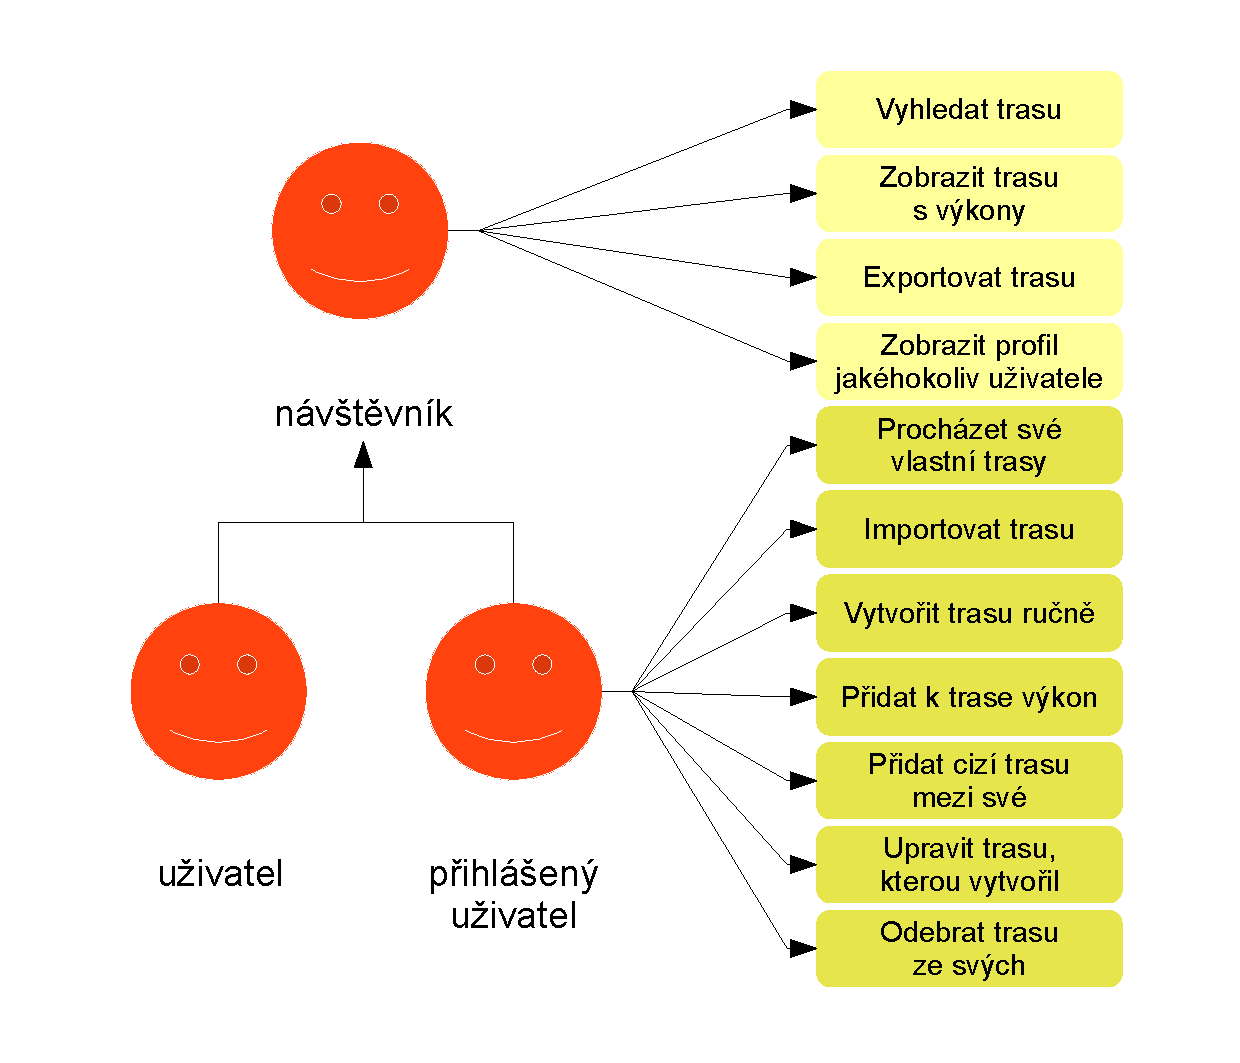
\includegraphics[width=\textwidth, keepaspectratio]{fig/use-case}
	\caption{Schéma případů užití.}
	\label{obrUseCase}
\end{figure}

\section{Uživatelské rozhraní}
V~návrhu uživatelského rozhraní jsem se inspiroval u~známých a
úspěšných služeb jako např. Flickr.com, Google.com nebo i český
Seznam.cz, kde se často soustředí jen na hlavní sdělení stránky a
jinak ponechávají uživateli volný prostor. Vzhled potom působí
přehledně, vzdušně a jednoduše a uživateli se s~ním pracuje lépe
\cite{design}. Pod těmito výrazy lze sice prezentovat i návrh, kde si
grafik jednoduchost vyložil minimální propracovaností prvků, ale
snažil jsem se, aby tato situace u~mé aplikace nenastala.

\begin{figure}[h]
	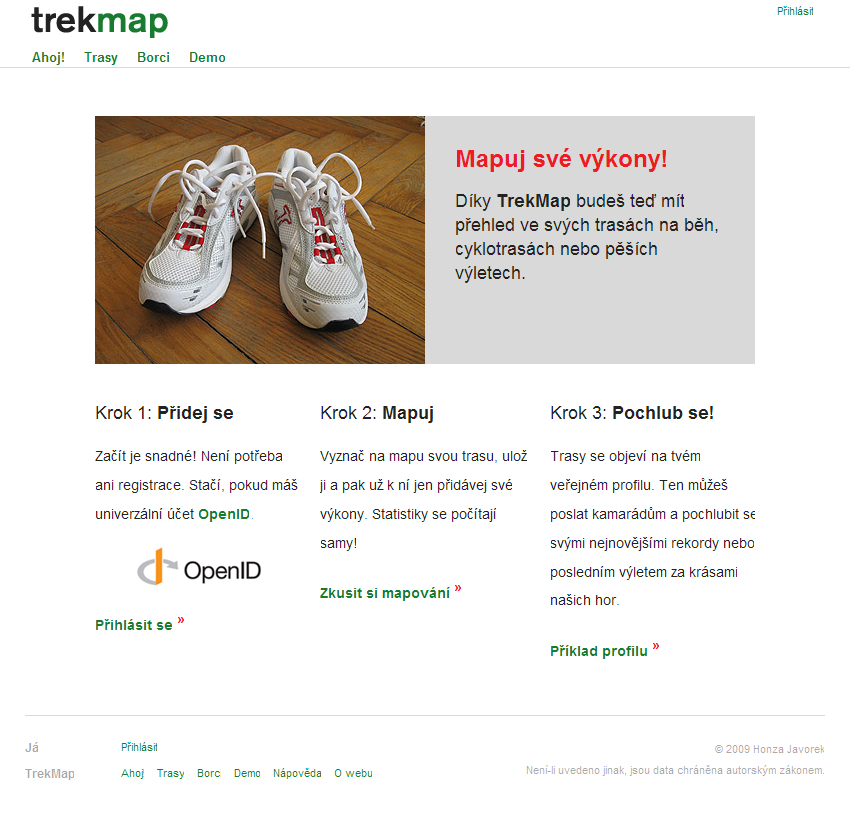
\includegraphics[width=\textwidth, keepaspectratio]{fig/screentexty}
	\caption{Úvodní stránka systému.}
	\label{obrTexty}
\end{figure}

\subsection{Texty}
V~rámci uživatelského rozhraní jsou velmi důležité texty. Měly by být
stručné, jednoznačné, srozumitelné a měly by uživatele vést k~akci
\cite{ui}. Významné je také navození atmosféry při komunikaci
s~uživatelem. Jak ukazuje trend nových internetových aplikací, nemusí
být vždy nutné zachovávat oficiální tón. Jestliže uživatel pracuje
s~informačním systémem, který spravuje jeho účetnictví a umožňuje mu
tisk faktur, očekává od něj i seriózní komunikaci. Pokud však
aplikaci využívá spíše ve volném čase, není špatným rozhodnutím
zvolit tón neformální a pokusit se navodit mezi aplikací a člověkem
přátelskou atmosféru \cite{informalTone}. V~rámci toho, aby aplikace
vyšla vstříc uživateli, jsem také implementoval do celého systému
údaj o~jeho pohlaví a všechny texty používají na jeho základě
korektní formulace. Jedinou vyjímkou je ne zcela formální výraz
\uv{borci}, který je dle platných pravidel přechylován jako
\uv{borkyně}, ale to mi subjektivně neznělo příliš přirozeně. 

\subsection{Navigace}
Hlavní menu má tři nebo čtyři položky pro přístup k~hlavním
oblastem aplikace. Další stránky, které nemusí mít uživatel tolik na
očích, jsem zpřístupnil pod podrobnější navigací v~patičce webu.
Hlavní menu nesplňuje známé pravidlo o~vyznačení aktuální pozice pro
lepší orientaci, protože uživatel se většinu času nachází pouze
v~oddíle {\it trasy} a zvýraznění tlačítka {\it borci} při přechodu na
vlastní či cizí profil by jej asi spíše jen mátlo.

\begin{figure}[h]
	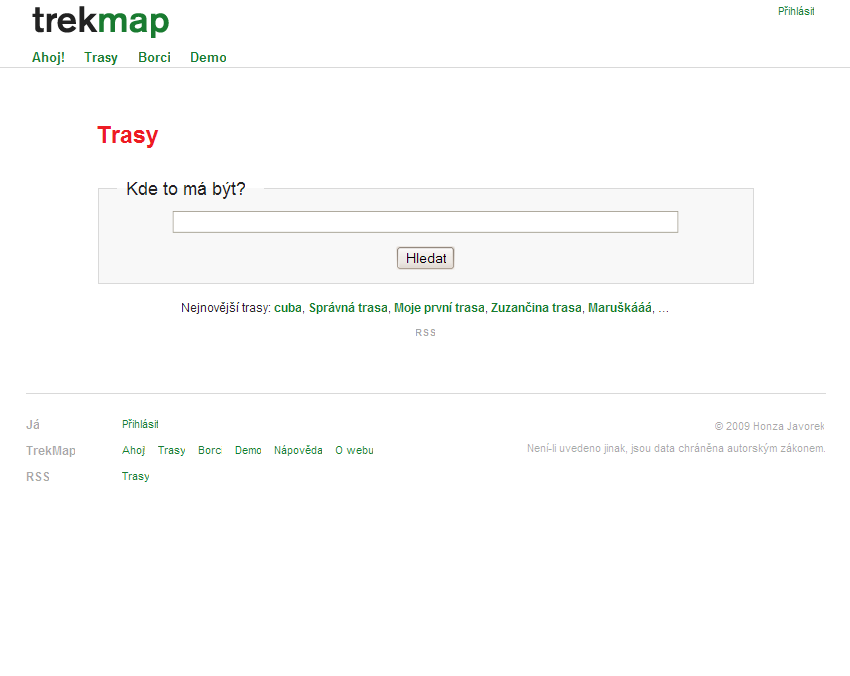
\includegraphics[width=\textwidth, keepaspectratio]{fig/screennav}
	\caption{Z~této obrazovky je dobře patrné umístění hlavního menu a
	podrobnější navigace v~zápatí webu. Na formuláři pro vyhledávání tras lze
	vidět přímost a jednoduchost komunikace s~uživatelem.}
	\label{obrGoogleMap}
\end{figure}

\subsection{Omezení chyb uživatele}
Systém by měl počítat s~tím, že uživatel bude (ve většině případů
nevědomky) chybovat. Může kliknout na tlačítko o~kousek vedle než
zamýšlel a omylem si smazat svůj rekordní výkon na trase nebo může
špatně vyplnit formulář a snažit se jej odeslat s~pro aplikaci neplatnými daty.

Ve všech nevratných případech užití jsem uživateli \uv{podstrčil}
potvrzovací dialog na bázi JavaScriptu (viz \ref{javaScript}). Ten
není sice spolehlivý, protože může být v~prohlížeči vypnutý, ale na
druhou stranu je celá mapová část aplikace založena právě na tomto jazyce,
takže lze předpokládat, že všichni návštěvníci pracující se svými
daty budou mít JavaScript povolen. V~případě formulářů je kontrola dat
navíc zdvojena -- operuje zde i serverová část, která za žádných
okolností neplatná data do databáze nepropustí a i v~případě
vypnutých skriptů vypíše chybová oznámení.

\section{Specifika práce na základě API}
Vystavět aplikaci z~větší části na externích zdrojích přináší možnost
využít již hotových, profesionálních a ihned funkčních řešení a služeb
od specializovaných poskytovatelů. Kdybychom si například chtěli sami
naprogramovat mapový systém, stálo by nás to nemalé prostředky a
rozsahem problému bychom překročili celou tuto práci. Stejně tak by
nebylo snadné zajistit si svá vlastní geografická data s~nadmořskými
výškami nebo aktuální informace o~počasí. S~použitím API se na tyto
problémy nemusíme soustředit a s~využitím minima úsilí spojujeme
existující prostředky do velmi silných aplikací.

Přístup samozřejmě ale přináší také nevýhody. Zdroje dat nejsou nijak
v~naší moci a proto hrozí riziko prodlev či nedostupnosti služeb
v~případě lepším, v~tom horším potom jejich neaktuálnost, chybovost, nebo
dokonce zánik. Prodlevy v~odpovědích z~cizích serverů musí program
zohlednit, zabývat se synchronizací požadavků s~interaktivním
uživatelským rozhraním a zamezit kolizím. Pokud navíc hrozí, že 
prodlevy budou dlouhé a znepříjemní uživatelský prožitek, je dobré
funkci, která je způsobuje separovat a dát uživateli možnost ji
vypínat a zapínat. Rizika s~vážným dopadem na funkčnost programu může
potom aplikace postavená nad API ošetřovat především omezením své
závislosti na jediném poskytovateli dat.

U~mapových podkladů si takové řešení můžeme představit například
v~naprogramování vrstvy, která nám poskytne rozhraní k~funkcím API,
ale oddělí nás od jejich konkrétní implementace. Vrstva potom může
obalovat API Google Maps, Mapy.cz i Amapy.cz (viz \ref{vybermap}) a
konkrétní službu potom použít na základě jediného parametru, podobně
jako se to dělá například u~databázových vrstev s~abstrakcí
několika druhů SŘBD (viz \ref{mysql}). Podobný projekt již existuje a
nese název Mapstraction\footnote{Aktuální zdrojové kódy jsou k~dispozici na
\url{http://code.google.com/p/mapstraction/}.}, ale je ve velmi ranném stádiu
a navíc podporuje zatím pouze globální
mapové systémy. Využití jeho zdrojových kódů a případné zanesení českých
mapových API je nyní tedy spíše zajímavou ideou do budoucna.

U~ostatních podkladů není omezování rizik tak obtížné. Pokud má
aplikace na výběr z~několika podkladů, může jednoduše použít lepší
z~nich a pokud ten selže, ve výjimce se na data dotáže alternativního,
byť třeba méně přesného. Takto jsem zdvojil například API pro
získávání nadmořské výšky (viz \ref{vyskovyProfil}). Pokud výběr
není, nejedná se většinou o~příliš významnou vlastnost a uživatel se
bez ní může obejít (např. vrstva s~kamerami).

\section{Databáze}
Ke znázornění dat v~databázi (viz \ref{mysql}) jsem využil
vyjadřovacích schopností tzv. {\it entity-relationship diagramu}. Ten znázorňuje svět jako
soubor entit a vztahů mezi nimi. Uzly znázorňují data v~podobě
entitních množin a hrany potom vztahy mezi nimi. Entitní množiny,
tedy skupiny entit stejného typu, mají své atributy (vlastnosti).
Jedna z~nich musí být vždy jednoznačný identifikátor, primární klíč.
Ve své aplikaci jsem prakticky vždy přistoupil ke speciálním číselným
identifikátorům, jež se samy navyšují v~posloupnosti přirozených
čísel.

\begin{figure}[p]
	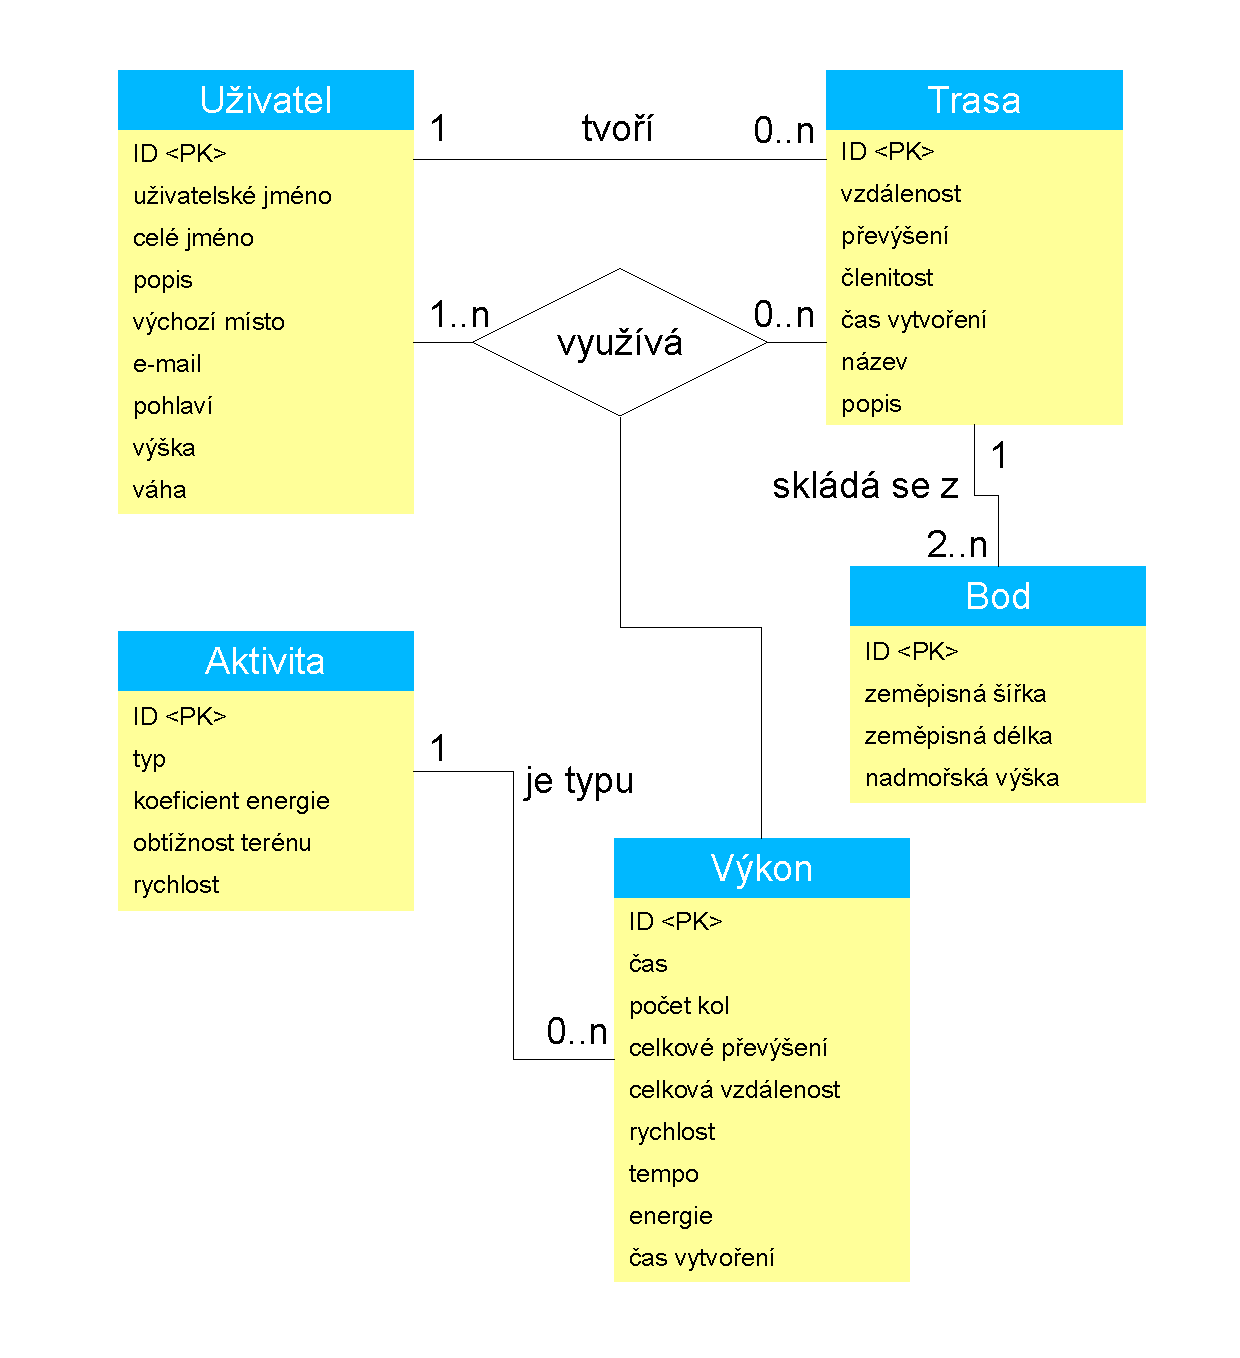
\includegraphics[width=\textwidth, keepaspectratio]{fig/erd}
	\caption{Entity-relationship diagram.}
	\label{obrErd}
\end{figure}

Do diagramu, jenž lze vidět na obrázku \ref{obrErd}, jsem nezahrnul samostatnou
entitní množinu pro instantní záložky z~dema aplikace, protože se
zbytkem aplikace nijak nesouvisí a ve své jednoduchosti
zřejmě nesplňuje ani první normální formu relace. V~tabulce se
nachází pouze identifikátor, serializovaná data uložené trasy a čas vytvoření
(záložky jsou aplikací po měsíci automaticky smazány).

Data o~uživatelích jsou z~části vyplňována samotnou aplikací díky
OpenID (automatická registrace, viz \ref{openid}), ale některá data musí
uživatel zadat sám, přičemž všechna jsou dobrovolná. Data tras obsahují
název, stručný popis a sadu číselných údajů předem vypočítaných před
uložením trasy z~interaktivní mapy. K~trasám se váže vždy množina
bodů, kterými je tvořena. Zde jsem se rozhodl pro kardinality, které
neuvažují možnost přiřazení jednoho bodu více trasám, ač je to
reálně možné. Uživatel mapu zadává interaktivně a body mají své
zeměpisné souřadnice ukládány v~přesnosti na několik desetinných
míst. Aby se sešly dva stejné je velmi málo pravděpodobné a i kdyby
se tak někdy stalo, databázi taková duplicita nezatíží.
Posledními množinami entit jsou výkony a typy aktivit. Tabulka
s~výkony udržuje vypočítané hodnoty. Výkon je neměnný v~čase,
takže je nutné pevně uložit např. i spotřebovanou energii. Pokud by
totiž uživatel v~budoucnu změnil svou váhu, změnila by se
spotřebovaná energie pro všechny předešlé výkony a to je samozřejmě
špatné chování aplikace. Množina aktivit je krátký výčet činností
jako {\it jízda na kole}, {\it běh} nebo {\it běžky}. K~nim jsou
přiřazeny koeficienty pro výpočet spotřebované energie. Protože ty
ale závisí na obtížnosti terénu a rychlosti, má vždy každá činnost
několik záznamů a hledá se v~nich ne zcela rutinním SQL dotazem (viz
\ref{statistiky}).

Všechny tabulky jsou v~databázi provázány referenčními integritními
omezeními\footnote{MyISAM, výchozí typ pro tabulky v~MySQL,
referenční integritní omezení sice nepodporuje, ale jiný vestavěný
režim, InnoDB, ano.}.

\chapter{Implementace}

\section{Vrstvy aplikace}
Architektura je založena na samostatných vrstvách, jež komunikují
mezi sebou. Na úrovni serveru lze program rozdělit do třech hlavních:

\begin{itemize}
	\item Správa přístupu k~persistentním datům, tzv. {\it model}. 
	\item Vykreslování uživatelského rozhraní, {\it view} nebo česky
	také {\it pohled}.
	\item {\it Řadič}, jednotka spravující požadavky uživatele. Podle
	použité architektury je nazývána buď {\it controller} nebo {\it presenter}.
\end{itemize}

Separace do takových samostatných modulů umožňuje provádět dodatečné
změny rychle a jednoduše, bez vlivu na zbytek celé aplikace, což je
velmi výhodné.

\begin{figure}[h]
	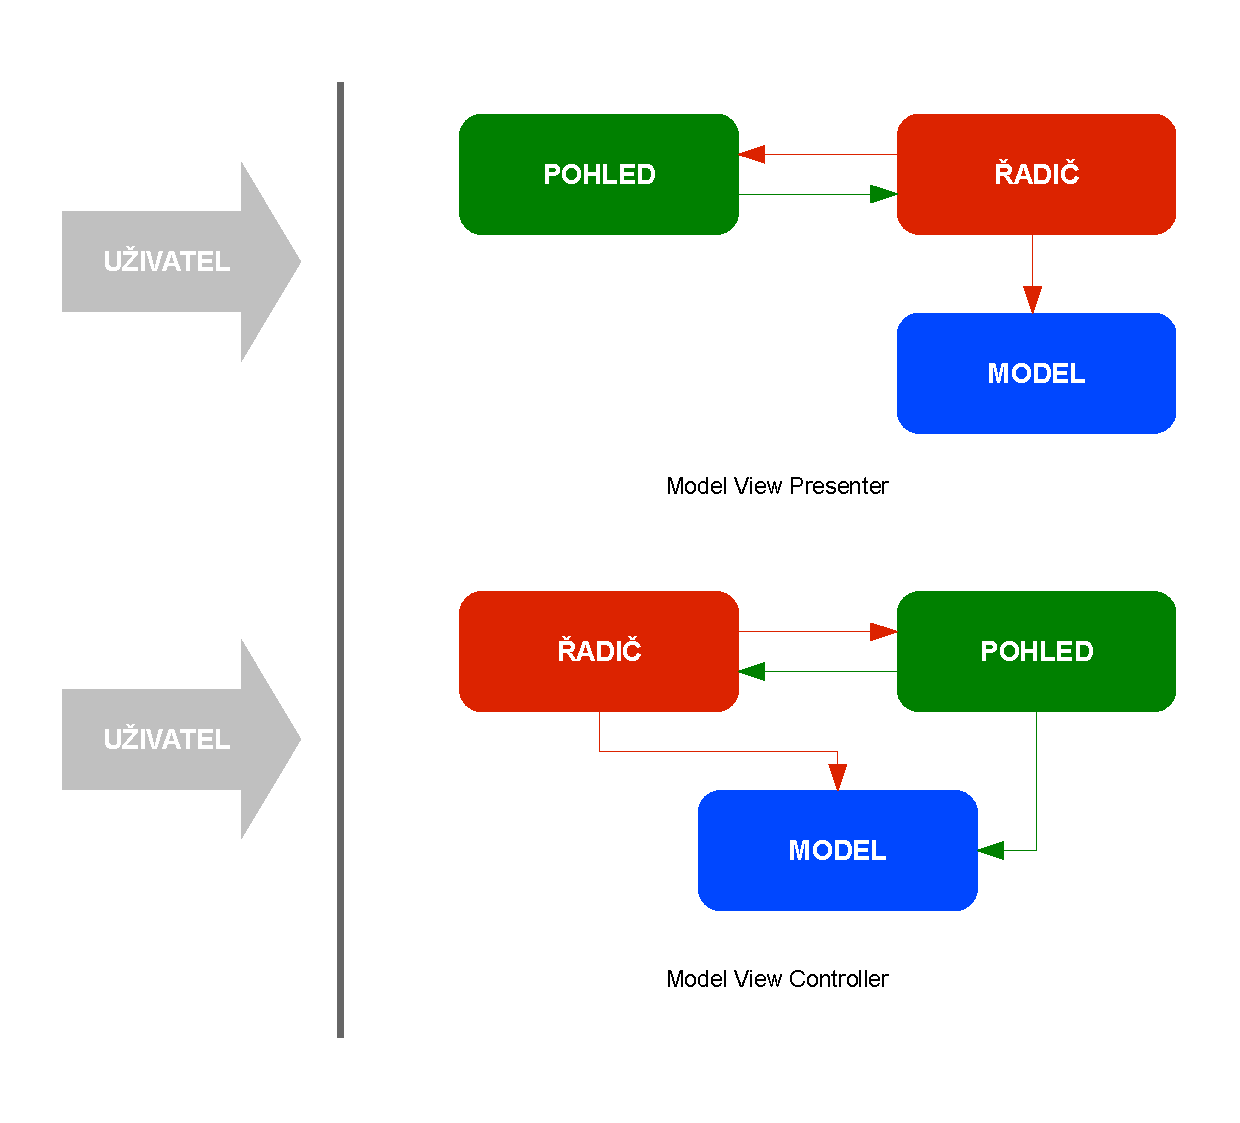
\includegraphics[width=\textwidth, keepaspectratio]{fig/mvp-mvc}
	\caption{Rozdíl mezi architekturami MVP a MVC. Zjednodušeno a
	přeloženo z~\cite{mvpNette}.}
	\label{obrMvpMvc}
\end{figure}

Jak lze vidět na obrázku \ref{obrMvpMvc}, propojení těchto tří vrstev je závislé
od použitého návrhového vzoru. Všeobecně známý a dnes populární je
vzor MVC (viz počáteční písmena anglických názvů vrstev), ale reálná
podoba dnešních webových aplikací se mu už právě v~oblasti propojení
vrstev spíše vzdaluje \cite{mvc}. Nette Framework (viz \ref{nette}),
který jsem na projektu použil se ve skutečnosti blíží spíše MVP \cite{mvp} a
k~architektuře MVC se hlásí jen jako ke \uv{spřízněné} \cite{mvpNette}.

Protože je velká část projektu napsána v~JavaScriptu, je nutné
aplikaci pojmout zároveň i z~ještě obecnějšího hlediska a rozdělit ji
na serverovou a klientskou vrstvu. Serverová, tedy PHP, generuje
uživatelské rozhraní a předává do něj data. Klientská část zastoupená
JavaScriptem s~těmito daty pracuje a na základě vstupů uživatele do
grafického rozhraní může posílat serveru zpět své vlastní asynchronní
požadavky a příkazy (viz \ref{ajax}).

Detaily rozdělení aplikace do vrstev MVC, resp. MVP, řeší vybraný
Nette Framework. Komunikace se serverem pomocí AJAXu je odstíněna jak
v~Nette, tak i v~JavaScriptovém frameworku MooTools. Obě tyto
problematiky jsou rozsáhlé a jejich objasňování je nad rámec této
práce, nicméně všechny podrobnosti by měly být zřejmé z~citovaných
zdrojů.

\section{Detaily řešení vybraných problémů}
V~následujícím oddíle jsem detailně popsal implementaci vybraných
problémů, které jsem při vývoji aplikace řešil.

\subsection{Mezidoménový AJAX}
Pro čtení dat z~API je důležité mít možnost poslat
z~JavaScriptu asynchronní požadavek ze serveru na server. Technologie
AJAX (viz \ref{ajax}) má bezpečnostní omezení, které skriptům
nedovoluje posílat požadavky na jiné servery, než na jakých právě
jsou. To lze řešit několika způsoby, z~nichž nej\-jednodušší je zřejmě
vytvoření {\it PHP proxy}, tedy přeposílacího skriptu na našem
serveru. AJAXová aplikace na něj pošle požadavek a v~parametru přidá
cíl požadavku. Náš skript na cíl vše přepošle a JavaScriptu vrátí
odpověď, které se mu ze vzdálené služby dostalo. Do svého proxy
skriptu jsem navíc vložil automatickou detekci formátu odpovědi a
její převod do JSON (viz \ref{json}), ať již je to v~původní odpovědi
třeba text nebo XML (viz \ref{xml}). Taková konverze usnadňuje
zpracování ve vlastním JavaScriptu, které lze napsat jednoduše a jednotně.

Některá API řeší propojení pomocí vkládaného JavaScriptového souboru
a různých {\it callbacků}, tedy zpětných volání námi definovaných
funkcí, jimž je předán výsledek dotazu na server přímo v~parametru.
To však situaci často jen komplikuje, jelikož je nutné namísto
standardních rutin pro AJAX připravit specializované a požadavky
často je pak nelze zasílat zcela instantně. Naprogramoval jsem tedy
v~JavaScriptu několik objektů obalujících tuto problematiku a ve zbytku
aplikace jsem přístup vykonával již jen přes toto rozhraní.

\subsection{Vykreslování objektů na mapu}\label{kresleni}
Vykreslování objektů na mapu usnadňuje samotné její API. Bez něj
by bylo velmi náročné podobnou funkčnost implementovat. Chceme-li
například vykreslit vektorovou spojnici bodů, předáme funkci z~API
map pouze pole bodů se zeměpisnými souřadnicemi a ta vše vykoná za
nás. Podobně jednoduše lze na mapu vykreslovat i ostatní prvky jako
značky nebo tzv. bubliny s~informacemi.

\begin{figure}[h]
	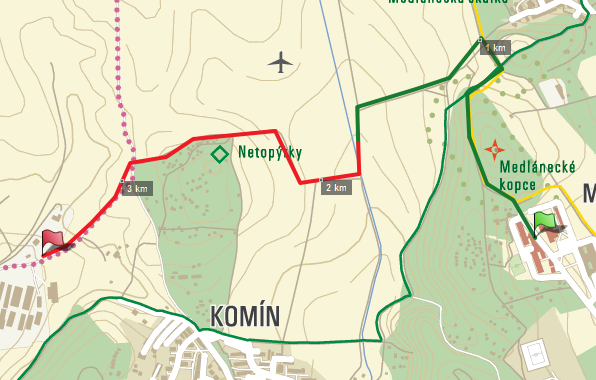
\includegraphics[width=\textwidth, keepaspectratio]{fig/screenline}
	\caption{Ukázka dvoubarevné spojnice.}
	\label{obrLine}
\end{figure}

Pro uživatelský komfort jsem implementoval netriviální vyznačení
trasy pomocí dvoubarevné spojnice. Barva se mění přesně v~polovině
délky trasy a pomáhá tak sportovci okamžitě vidět například od jakého
místa se již vrací zpět, pokud běží okruh. Polovina trasy je
detekována tak, že skript prochází postupně všechny segmenty trasy a
porovnává jejich vzdálenost od prvního bodu s~polovinou celkové délky
trasy. Dokud není v~polovině, ukládá body do jednoho pole (cesta tam)
a poté dopočítá přesný střed trasy ze souřadnic nej\-bližších bodů metodou
podobnosti trojúhelníků. Tento střed uloží jako koncový bod prvního
pole a zároveň i jako první bod nového pole pro cestu zpět. Do té
vloží všechny ostatní body trasy.

\subsection{Tématické vrstvy s~velkým množstvím značek}\label{vrstvy}
Tématické vrstvy jsou postaveny všechny na téže šabloně. Vstupem je
většinou buď přímo bod středu mapy a vzdálenost, v~jaké se mají
nalezené prvky hledat, nebo ohraničení oblasti pomocí
nej\-severovýchodnější a nej\-jihozápadnější souřadnice. Objekt vrstvy
v~klientském skriptu aplikace získá přes AJAXové API seznam bodů
s~případnými dalšími daty, které má zobrazit na mapě. Postupně si na
jejich základě vytvoří pole značek a to potom pomocí optimalizované
metody pro rychlé nahrání velkého množství značek (ta je přímo v~API
Amapy.cz) vloží najednou do mapy.

\begin{figure}[h]
	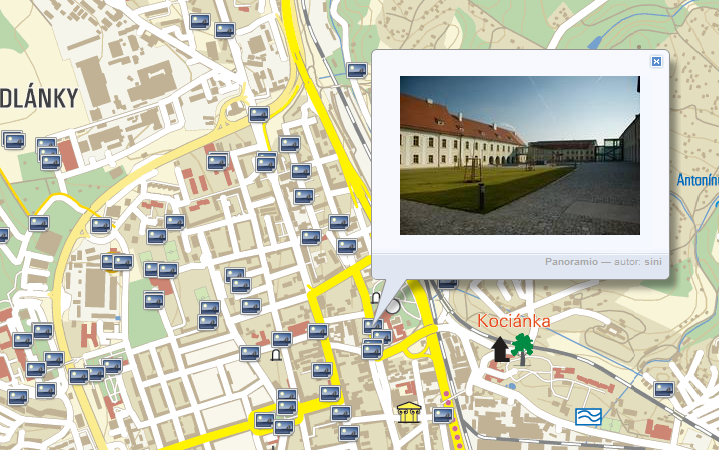
\includegraphics[width=\textwidth, keepaspectratio]{fig/screenlayer}
	\caption{Ukázka vrstvy se značkami.}
	\label{obrLayer}
\end{figure}

Jedinými dalšími problémy jsou potom řešení přepínače vrstvy a
postupné načítání značek. Přepínač je poměrně jednoduchá funkce,
která projde všechny značky a buď je schová, nebo naopak zobrazí (pro
to je podpora přímo v~API~Amapy.cz).

Načítání značek lze pohodlně řešit navázáním události na změnu výřezu
a měřítka mapy. Při každé takové změně se zavolá funkce, která získá
ze serveru nová data a zobrazí je na mapu. V~té chvíli někdy
vzniká problém, kdy server v~odpovědi pošle i prvky, které jsme již
na mapu nechali zobrazit dříve. Řešením je ukládat si značky do
asociativního pole pod řetězcem tvořeným spojením souřadnic bodu a
poté vždy kontrolovat, jestli přidávaný bod již v~poli (a tím tedy i
na mapě) neexistuje.

V~celé problematice vrstev značek je asi nej\-obtížnější zorientovat se
v~pořadí a vztazích funkcí v~rámci událostmi řízené architektury mapy
na jedné straně a AJAXu na straně druhé.

\subsubsection{Zobrazování značek typu POI}
Značky zájmových bodů (viz \ref{poi}) získávané z~GeoNames.org mají
mnoho kategorií a ještě větší škálu podtypů\footnote{Seznam všech
kódů je dostupný na \url{http://www.geonames.org/export/codes.html}.}.
Můžeme tak podle odpovědi ze serveru snadno dle speciálních kódů
rozlišit, zda jde o~horu, město, jezero, přírodní, architektonickou
či technickou památku. Rozlišení těchto typů by však po aplikaci
vyžadovalo rozsáhlou překladovou tabulku, podle níž by se mohl vypsat
detailnější český popisek nebo např. jiná značka. Jiné řešení by
mohlo také tento datový zdroj rozdělit do více různých vrstev a
umožňovat samostatně zobrazovat hory, samostatně města apod. V~obou
případech jsem považoval takové možnosti za rozšíření nad rámec této
práce, ale také za zajímavý směr rozvoje aplikace do budoucna.

\subsection{Zobrazování vzdálenosti na trase}
Implementace zobrazování vzdálenosti na trase přímo
v~mapě je v~podstatě kombinací znalostí z~oddílů \ref{kresleni} a
\ref{vrstvy}. Podobnou metodou s~použitím podobností trojúhelníků jako
při rozdělení vlastní spojnice na poloviny podle barev se počítají
jednotlivé vzdálenosti na trase a stejnými technikami jako při
zobrazování vrstev značek na mapu se na vypočítaná místa usazují
kilometrovníky. Intervaly pro zobrazení kilometrovníků je dobré určovat
na základě právě používaného měřítka.

\begin{figure}[h]
	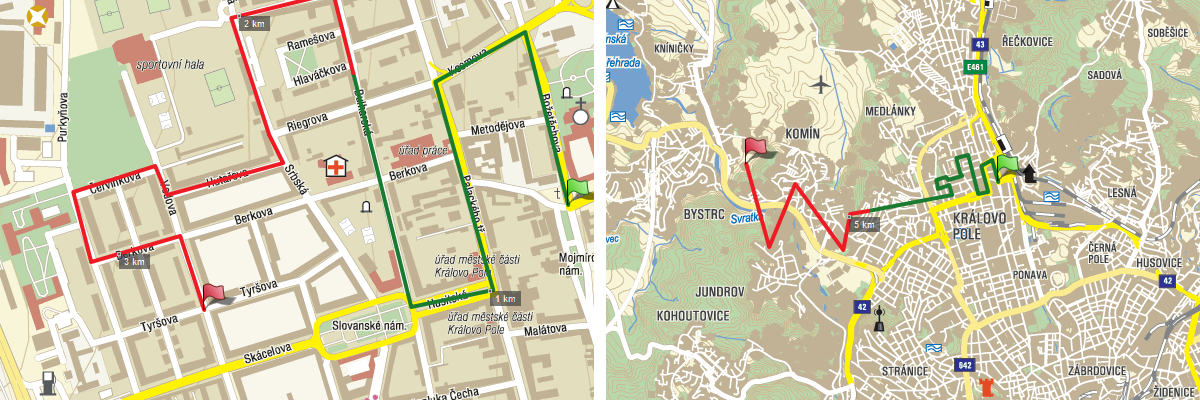
\includegraphics[width=\textwidth, keepaspectratio]{fig/screenmilestones}
	\caption{Kilometrovníky a dynamická změna jejich intervalu.}
	\label{obrMilestones}
\end{figure}

\subsection{Editor mapy}
Editor mapování trasy jsem koncipoval jako dvourežimový. Skládá se
z~několika tlačítek a jednoho hlavního, které režimy přepíná. Mapa se
tedy může nacházet ve dvou stavech, z~nichž první je určen jen pro
její prohlížení a druhý pro editaci trasy. Podle těchto módů se
vykreslují i tlačítka. Uživatel se mezi režimy může přepínat svobodně
a např. pokud se zabývá tvorbou trasy a přepne se do režimu
prohlížení, po návratu zpět do editačního může bez jakýchkoliv zábran
v~úpravách pokračovat. Podle uživatelského testování, které jsem
provedl na několika přátelích, nemají lidé s~pochopením tohoto
komplexního ovládacího prvku problém.

\begin{figure}[h]
	
\includegraphics[width=\textwidth, keepaspectratio]{fig/screeneditor}
	\caption{Ovládací panel editoru. Vlevo je stav při prohlížení mapy,
	vpravo v~režimu úprav.}
	\label{obrMilestones}
\end{figure}

Tlačítka se vykreslují s~HTML atributem {\tt disabled} vždy,
kdy není správná chvíle k~jejich stisknutí. Tento atribut znemožňuje
jejich použití. Každá akce na tlačítku má svou validační funkci a ta
je při každém překreslení editoru volána. Většina akcí například
nelze provést, pokud máme na trase pouze jediný bod (minimum jsou
dva, kdy vznikne první spojnice). Protože jsou tlačítka obrázková a
prohlížeče někdy nereagují po přidání atributu {\tt disabled}
zšednutím obrázků uvnitř tlačítek, je toto chování simulováno
JavaScriptem, kde je těmto elementům {\tt img} přiřazován efekt
částečné průhlednosti.

Dostupné akce jsou následující:

\begin{itemize}
  \item Vymazat,
  \item zpět,
  \item spojit do okruhu,
  \item stejnou cestou zpět,
  \item vidět celou trasu,
  \item uložit.
\end{itemize}

Pro akci pro zobrazení celé trasy v~nej\-vhodnějším vystředění
a přiblížení mapy je funkce přímo v~API~Amapy.cz. Tlačítko pro
uložení trasy je obslouženo metodou, která připraví trasu pro uložení
v~databázi a poté ji pošle přes AJAX do PHP, aby akci vykonalo. Při
úspěšném uložení PHP vrátí JavaScriptu v~odpovědi adresu, na kterou
má uživatele přesměrovat. Díky tomuto systému lze použít tytéž
komponenty pro vnitřní editor mapy i pro veřejné demo aplikace,
v~němž se trasy ukládají jinak, do jednoduchých záložek.

\subsection{Výškový profil}
Stavba výškového profilu je jeden z~nej\-obtížnějších úkolů projektu.
Je nutné zajistit data s~nadmořskou z~celé trasy a poté je zpracovat
do podoby spojnicového grafu.

Při zaznamenávání dat je důležité si uvědomit, že pokud známe
nadmořskou výšku dvou bodů, neznamená to, že mezi nimi existuje
lineární spojnice (např. mezi body Praha a Brno jistě nebude jen
pozvolné stoupání vyrovnávající rozdíl nadmořských výšek těchto
měst). Správně by měl systém dopočítávat mezibody na relevantních
intervalech a zjišťovat nadmořskou výšku i na nich. To však vede
k~velkému provozu na API pro zjištění výškopisu a také k~velkým
prodlevám. Naštěstí má Výškopis.cz (viz \ref{vyskopis}) pro zjištění
nadmořské výšky metodu pro hromadné zjištění bodů, takže lze tyto
problémy obejít. Kdybych mohl využít jen API od GeoNames.org, které
podporuje pouze zjištění nadmořské výšky z~jednoho bodu, situace by
se velmi zkomplikovala. 

Prodlevy ze získávání výškových dat nejsou velké, ale i kvůli zatížení
serverů s~API je vhodné dát uživateli najevo, že by měl chvíli
posečkat a na mapu neklikat. Vytvořil jsem tedy systém tzv. zámku
mapy. Jakákoliv funkce jej může využít a dokud je mapa zamčená,
překryje se poloprůhledným filmem po celé své ploše. Na ten potom
automaticky směřují všechna kliknutí uživatele a ztrácejí tak účinek.
Abych takový stav aplikace uživateli ozřejmil, nastavil jsem
překryvné vrstvě ve stylech (viz \ref{css}) kurzor do \uv{čekající}
podoby.

Data o~výškách se ukládají jak k~jednotlivým bodům trasy, tak i pro
jednotlivé segmenty mezi nimi. Zde je na základě vzdálenosti mezi
dvěma body počítán vhodný interval a v~něm se potom provádí měření
nadmořské výšky. Je dobré nastavit minimální možný interval (např.
50 nebo 100 m), aby se aplikace nepokoušela dotazovat API na
zeměpisných souřadnicích, které jsou jen pár metrů od sebe.

\begin{figure}[h]
	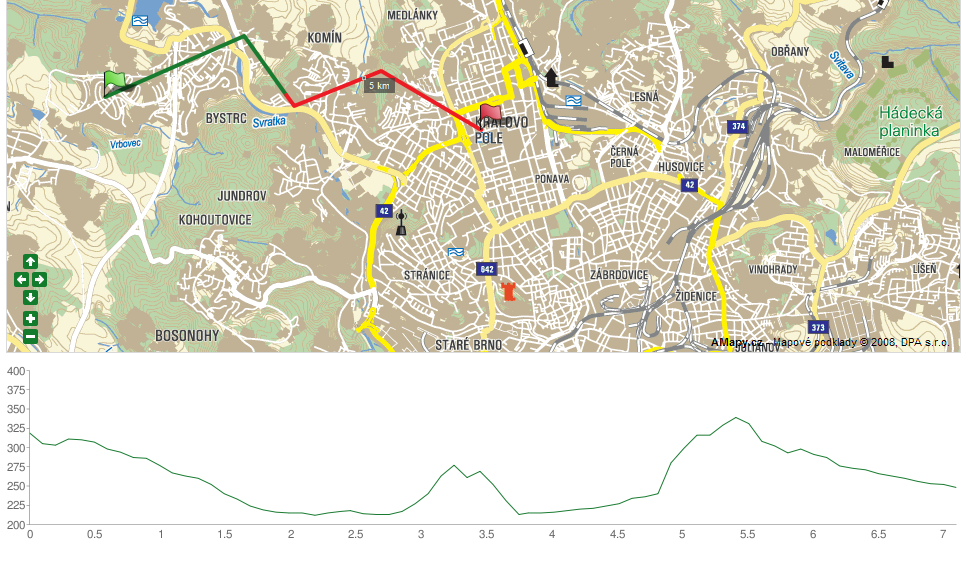
\includegraphics[width=\textwidth, keepaspectratio]{fig/screenaltitude}
	\caption{Ukázka výškového profilu trasy.}
	\label{obrAltitude}
\end{figure}

Vzniklá řada výškopisných hodnot po délce celé trasy je potom
podkladem pro vykreslení grafu. Jelikož API pro jeho tvorbu
(viz \ref{grafy}) je velmi jednoduché, je nutné ještě data před
odesláním připravit -- převést je do relativních procentuálních
hodnot a především nechat pole hodnot prořídnout, aby se jich na
vzdálený server neposílalo více než několik málo set. Z~většího počtu
stejně většinou nelze vykreslit v~síti pixelů na obrazovce přesnější
graf.

\subsection{Vyhledávání polohy a trasy podle zadaného místa}
Vyhledávání polohy na mapě v~editoru je obsluhováno pomocí geocodingu
(viz \ref{geocoding}). Pokud uživatel zadá do textového pole místo a
odešle jej, JavaScript se přes API zeptá na jeho zeměpisné souřadnice
a první výsledek odpovědi zacílí na mapě. Odpověď ze vzdáleného
serveru jsem pomocí parametrů upravil na ryze českou, aby nemohly vznikat
konflikty (např. obec s~názvem Praha existuje několikrát po celém
světě), takže např. na heslo {\it New York} je uživateli zobrazeno
upozornění, že místo nelze najít.

Geocoding je využit i při hledání tras. Rozdíl je ve skutečnosti, že
vzdálené API tentokrát volá přímo PHP a výsledek nepředává do
prezentační vrstvy, ale přímo podle něj vyhledává v~databázi. Zde
jsem narazil na jeden z~nej\-obtížnějších problémů aplikace, ač
v~dnešní době projektů založených na mapách by měl být velmi často
řešený. Body trasy jsem do databáze uložil jednotlivě proto, aby
v~nich šlo hledat právě způsobem, kdy jsou vůči zadaným souřadnicím v~SQL dotazu
porovnávány. Jejich seřazením od nej\-bližších a zároveň zmenšením
výsledku SQL dotazu na záznamy s~unikátními trasami lze potom
dosáhnout seznamu tras nej\-bližších k~požadovaným souřadnicím. Způsob,
kdy se hledá ve všech bodech trasy má výhodu v~tom, že najde všechny
trasy v~blízkosti bez ohledu na to, kde začínají. Pokud bude
například existovat cyklistická trasa, která začíná v~Olomouci,
pokračuje až k~Brnu a vrátí se zpět, systém by ji podle startovního
místa na dotaz {\it Brno} nevyhledal. Prohledávají-li se však všechny
body trasy, může ji najít dokonce i jako bližší než jinou trasu
z~okolí Ivančic, jejíž body jsou ve skutečnosti dál.

Velký problém však vzniká přímo v~řešení porovnání blízkosti bodů
v~SQL dotazu. Na výpočet vzdálenosti dvou bodů podle zeměpisných
souřadnic, která je udána v~kilometrech, existuje velmi složitá
rovnice. Implementujeme-li ji jako běžný dotaz,
můžeme výsledky dostávat i v~řádech několika sekund
\cite{distanceSearch}. Řešením je použití uložené procedury přímo
v~databázi, ale při pokusu o~takovou věc jsem se potýkal s~velkými
problémy při využití procedury MySQL v~dotazech volaných z~PHP.
Nakonec jsem se rozhodl pro méně přesné, ale velmi snadné
alternativní řešení. Podle nalezeného kalkulátoru Federace Amerických
Vědců\footnote{Dostupný na
\url{http://www.fas.org/news/reference/calc/degree.html}.} jsem
jednorázově přepočítal vzdálenost jednoho stupně v~zeměpisné šířce i
v~zeměpisné délce na kilometry a dle těchto převodních hodnot
v~databázi aplikace vyhledává. Stupně sice nelze přepočítat na
kilometry v~globálním smyslu, ale lze to udělat na základě zadané
zeměpisné šířky. Protože je naše země malá a projekt se zaměřuje
pouze na ČR, není chybou vypočítat si hodnoty předem pro zeměpisnou
šířku, na které se stát nachází a použít je v~aplikaci. Podle
výsledků vyhledávání lze usoudit, že tato volba nebyla špatným
krokem, protože problém je v~kontextu aplikace vyřešen a zároveň
s~minimálními nároky.
Pro studium detailů sofistikovanější cesty jak řešit tento problém
pomocí výpočtu vzdálenosti v~databázové proceduře doporučuji výbornou
prezentaci pana Rubina ze společnosti MySQL AB, citovanou výše.

\subsection{Demo aplikace}
Aby si návštěvníci webu mohli aplikaci nej\-dříve vyzkoušet a potom se
rozhodnout, zda ji chtějí používat, připravil jsem demo. To má zcela
totožný mapový editor i ostatní funkce jako po přihlášení, akorát
trasy v~něm vytvořené nelze uložit do systému, ale pouze jako
instantní záložku. Pokud uživatel stiskne tlačítko pro uložení, PHP
server nechá trasu serializovanou ve formátu JSON (viz \ref{json}),
přidělí jí jednoznačný identifikátor a uloží do jednoduché tabulky
v~databázi. Uživateli je následně sdělena adresa, na níž svou trasu
může zpětně najít. Záložka je veřejně zobrazitelná a je dostupná měsíc
-- u~každého záznamu v~tabulce je datum jeho vytvoření a při každém
vložení nového se smažou všechny záznamy starší než právě jeden
kalendářní měsíc.

\subsection{Rozlišení pohlaví uživatele}
Rozlišení na muže a ženu probíhá jednoduše. Pokud OpenID poskytne
systému informaci o~pohlaví, nastaví ji v~databázi automaticky.
Uživatel má ve svém nastavení možnost tuto volbu měnit. Pokud by jeho
příjmení mělo koncovku {\it -ová} a měl pohlaví nastaveno na {\it
muž}, je upozorněn, že jeho údaj o~pohlaví je možná nesprávný.
Pohlaví je rovněž rozlišeno pomocí výchozích obrázků uživatelů.

\subsection{Výpočet statistik}\label{statistiky}
Pro výpočet statistik trasy a uživatele se používají většinou poměrně
známé vztahy. Pro úplnost je zmiňuji v~následujícím přehledu:

\subsubsection{Délka trasy}
Délku vypočítáme součtem vzdáleností všech segmentů trasy.

\subsubsection{Převýšení na trase}
Převýšení je součet rozdílů nadmořských výšek na všech částech trasy,
kde sportovec stoupá a překonává tedy větší zátěž.

Implementace statistik převýšení je v~aplikaci nedokonalá, protože už
z~charakteristiky této hodnoty vyplývá, že je rozdílná v~obou směrech
trasy. Pokud by se např. běžec trasu rozhodl absolvovat v~opačném
směru, nemá možnost si v~systému tento směr nastavit a údaje
o~převýšení jeho výkonu nebudou správné. Toto chování by tedy mělo
být v~budoucnu vylepšeno.

\subsubsection{Členitost trasy}
Tato statistika je důležitá pro výpočet energie spotřebované při
výkonu. Členitostí se chápe rozdíl nej\-menší a nej\-větší nadmořské
výšky v~oblasti. Určení takové oblasti není zcela triviální
geodetický úkol, ale zde máme oblast jasně určenou trajektorií trasy,
takže lze tento problém obejít jednoduše použitím výškopisných hodnot
pouze z~trasy.

\subsubsection{Vzdálenost překonaná při výkonu}
Vypočítáme jako $d = D \cdot k$, kde $D$ je délkou
trasy a $k$ počtem kol, jež sportovec absolvoval.

\subsubsection{Převýšení během výkonu}
Vypočítáme obdobně, tedy jako $p = P \cdot k$, kde $P$
je převýšením trasy v~patřičném směru a $k$ počtem kol, jež
sportovec absolvoval.

\subsubsection{Rychlost výkonu}
Rychlost lze vypočítat rovnicí $s = \frac{d}{t}$, kde $d$
je vzdálenost překonaná při výkonu a $t$ čas. Uživatel
zadává čas jako trojici čísel představující hodiny, minuty a sekundy. Ten je potřeba
převést do jedné z~těchto jednotek a následně počítat
s~korespondující jednotkou vzdálenosti (tedy km a h, m a s).

\subsubsection{Tempo výkonu}
Tempo připomíná rychlost v~převráceném zlomku, protože jej lze
získat jako $p = \frac{t}{d}$, kde $d$ je vzdálenost
překonaná při výkonu a $t$ čas, ale při přípravě hodnot do
vzorce nesmíme zapomenout, že zde je všeobecně používanou jednotkou
tzv. {\it minuta na kilometr}. Musíme tedy hodnoty hodnoty dělit jako
$\frac{min}{km}$.

\subsubsection{Energie spotřebovaná při výkonu}
Energii lze vypočítat na základě vztahu $E = k~\cdot t \cdot m$, kde
$k$ je koeficient v~jednotkách $kJ / kg \cdot min$,
$t$ je čas výkonu zátěže v~minutách a $m$
hmotnost sportovce. Koeficient je tabulková hodnota závislá na typu
terénu a rychlosti sportovce.

Sesbírané tabulkové hodnoty jsou uloženy do samostatné tabulky
v~databázi. Každý záznam má navíc údaj o~názvu aktivity, typu terénu a
rychlosti sportovce. Uživatel pro svůj výkon v~grafickém rozhraní
vybere název aktivity. V~jediném SQL dotazu jsou vyhledány všechny
záznamy, které mají přiřazen tento název a z~nich je vybrán ten,
který splňuje kategorii terénu a má rychlost sportovce nej\-bližší
číslu, jež jsme si na základě uživatelova výkonu již spočítali.
Kategorizaci terénu jsem vyřešil počítáním členitostí tratí a určením,
zda s~takovou členitostí spadá do rovinatého, středně kopcovitého
nebo obtížného kopcovitého terénu. Hranice těchto tří skupin jsem
určil subjektivně dle vlastních běžeckých zkušeností, avšak na
pevném základě geomorfologického členění typů georeliéfů (tj. roviny,
pahorkatiny, vrchoviny, hornatiny a velehornatiny v~závislosti na
číselném vyjádření členitosti oblasti).

\subsubsection{Index tělesné hmotnosti}
Index tělesné hmotnosti, označovaný také jako {\it body mass index}
nebo i zkratkou BMI, je číslo používané ve statistice jako měřítko
obezity. Nelze aplikovat přímo na jedince, protože určení jeho stavu
je v~tomto ohledu velmi individuální (např. kulturista s~velkým
množstvím svalové hmoty může mít hodnoty jako by byl obézní). Usoudil
jsem však, že jako orientační hodnota se může uživatelům aplikace
hodit a její zobrazení jsem zahrnul přímo k~nastavení výšky a váhy
uživatele.

Hotnota lze vypočítat vzorcem $BMI = \frac{m}{h^2}$, kde
$m$ je hmotnost uživatele v~kilogramech a $h$ jeho výška
v~metrech.

\subsection{Detaily exportu a importu dat}
Oba formáty GPX i KML (viz \ref{importExport}) jsou založeny na
jazyce XML, takže lze import dat unifikovat.

Jazyk PHP má pro rozbor XML rozhraní, jež podle své jednoduchosti dostalo i jméno
-- {\it SimpleXML}. Předaný řetězec nebo soubor rozebere jediná funkce
okamžitě do stromu objektů (využívá tedy DOM, viz \ref{dom}), s~nímž
lze pak dále pracovat nejen tradičními funkcemi pro objekty, ale
např. přímo v~PHP i pomocí XPath, dotazovacího jazyka nad XML
soubory. Těmito metodami není po prostudování specifikací elementů
obou formátů obtížné importovaný soubor rozebrat a složit z~dat svou
vlastní datovou jednotku trasy. Problém nastává ve chvíli, kdy chceme
takovou trasu poslat AJAXem z~JavaScriptového editoru do PHP. GPS
navigace nebo jiné nástroje pro tvorbu tras totiž vytvářejí obrovské množství
bodů za účelem přesnosti trasy. Při zmíněném přenosu narazíme na
problém, kdy vzniklý řetězec přesahuje podporovanou délku HTTP metody
GET a není možné data odeslat. Tento problém může vzniknout
teoreticky i při ukládání trasy uživatelem, ale je to mnohem méně
pravděpodobný stav. V~obou případech by však bylo dobré do
budoucna problém řešit buďto kódováním dat do úspornější podoby,
posíláním dat po dávkách nebo vyvarováním se problému jinou architekturou případu užití
aplikace. Ve svém projektu jsem zatím zavedl metodu pro rovnoměrné
snížení počtu bodů, ale ta není příliš vhodná, protože zjednodušená
trasa se od původní liší více, než by mohlo být přijatelné.

Export dat oproti importu žádné problémy neobnáší a jedná se pouze
o~vsazení patřičných proměnných do šablony pro XML soubor. Ten je
potom vyhodnocen a poslán na výstup s~MIME typem, jenž přísluší
vybranému formátu. To je {\tt application/vnd.google-earth.kml+xml}
v~případě KML a obecné {\tt application/xml} pro GPX, protože to nemá
přiřazen svůj vlastní oficiální MIME typ.

\chapter{Vývoj a testování}
Systém byl vyvíjen v~univerzálním vývojovém prostředí Eclipse~3.4.2 za
využití rozšíření pro práci s~PHP (PDT~2.0), SVN (Subclipse~1.4) a
JavaScriptem (Aptana~1.5).

Použity byly frameworky Nette~Framework~0.9, a MooTools~1.11. Verze
JavaScriptového frameworku přitom v~době psaní aplikace byla vyšší,
ale zde byl projekt závislý na té verzi, jež poskytuje delší dobu
neudržované API~Amapy.cz.

Aplikace byla vyvíjena a testována na PHP~5.2.5 a MySQL~5.0.45.
Grafické uživatelské rozhraní bylo přizpůsobeno prohlížečům
Mozilla Firefox~3, Opera~9, Safari~3 (prohlížeč pro produkty Apple),
Google Chrome~2 a Internet Explorer ve verzích 7 i 8. Stále ještě
dominantní prohlížeč na trhu (ač ustupující), Internet Explorer~6,
není oficiálně podporován, protože jsem ve svém okolí nenarazil na
systém, kde by byl k~dispozici. Nové verze tohoto programu se šíří
automatickými aktualizacemi operačního systému MS~Windows a návrat ke
starým verzím není možný. Řešením do budoucna by mohla být instalace
speciálního softwaru pro virtualizaci operačního systému MS~Windows a
ten mít ve verzi, která Internet Explorer~6 obsahuje.

\chapter*{Závěr}
Cílem práce bylo pokusit se vytvořit systém, v~němž je řešena
architektura mashupu, tedy relativně jednoduché aplikace založené na
práci s~daty od jiných, externích poskytovatelů pomocí jejich API.
V~tomto konkrétním případě šlo o~nej\-typičtějšího zástupce takové
architektury, mapový projekt. Zadání se zaměřilo na vývoj aplikace,
v~níž si, ve stručnosti sděleno, může uživatel pohodlně s~pomocí mapy
vytvořit trasu svého běhu nebo jízdy na kole, tu si uložit a mít
následně k~dispozici statistiky trasy či svého výkonu. Jako doplňková
funkce bylo zmíněno také sdílení těchto dat s~jinými uživateli. Cíl
této práce byl tedy dosažen a zadání splněno.

\section*{Význam práce}
Tvorba projektu pro mne měla značný význam, protože jsem
mohl v~praxi využít nejen vědomosti dlouho nabývané v~oblastech informačních systémů a webových
aplikací, ale také například znalosti z~jiných oborů jako jsou
signály a systémy (to když jsem potřeboval snížit počet bodů pro graf
výškového profilu). Za nej\-cennější však považuji svůj obrovský posun
ve znalostech jazyka JavaScript, jenž má odpovědnost za jádro celého
projektu. Jelikož mám s~programováním webových aplikací už praktické
zkušenosti, byl jsem při tvorbě systému rád, že neřeší příliš mnoho
rutinních problémů z~vývoje pro web a že naopak do této oblasti
přináší spíše nové otázky a pro webového vývojáře neotřelou
problematiku ležící na cestě ke geografickým informačním systémům.

\section*{Budoucnost projektu}
Další vývoj projektu lze vyvodit z~doporučení, která jsem
postupně zmiňoval již v~průběhu práce. Do budoucna je
nutné některé funkčnosti po zkušenostech s~jejich implementací znova
analyzovat a jejich problematiku řešit jinak -- efektivněji nebo
s~ohledem na vyhnutí se určitým těžkostem a nedokonalostem. Aplikace
jako celek rozhodně nepůsobí jako slepá ulička ve vývoji a celý
projekt jsem se snažil koncipovat ne jako cvičení, ale jako
zcela životaschopný a použitelný v~praxi, takže by mělo být
možné najít motivaci (např. obchodní model) k~jeho dalšímu rozvoji.

Navrhoval bych se v~budoucnosti zaměřit na následující:

\begin{itemize}
  \item Nalézt nebo si počkat na vhodnější API lokálních map.
  \item Propracovat lépe komunikaci mezi PHP a JavaScriptem.
  Sjednotit přístup a vytvořit jednotnější rozhraní, které by později
  mohlo být i veřejně otevřeno (aplikace sama by se tak mohla stát
  poskytovatelem vlastního API).
  \item Zavést pro uživatele možnost ukládat si k~trasám své vlastní
  poznámky, fotografie, značky\ldots Umožnit export těchto dat do GPX
  a KML.
  \item Vyřešení problematiky zpětné editace trasy (narušení
  konzistence s~existujícími výkony) například možností trasu
  kopírovat a následně upravit. Implementovat mocnější editor trasy,
  který podporuje zpětné úpravy dílčích úseků trasy (např. přesunutí
  bodu uprostřed spojnice trasy na jiné místo, přidávání a odebírání
  bodů, aj.).
  \item Profil uživatele obohatit o~statistiky uživatele, komentáře a
  aplikaci celkově vybavit více sociálními funkcemi podporujícími
  tvorbu uživatelské komunity.
\end{itemize}
